
\section*{CHƯƠNG 2. THIẾT KẾ CHI TIẾT HỆ THỐNG}
\setcounter{section}{2}
\setcounter{subsection}{0} %LƯU Ý MỖI LẦN THÊM CHƯƠNG MỚI CẦN THÊM CÂU NÀY ĐỂ RESET THỨ TỰ CỦA SUBSECTON VỀ 1
\setcounter{table}{0} % LƯU Ý SAU MỖI LẦN GỌI BẢNG HAY HÌNH ẢNH PHẢI THÊM CÂU NÀY ĐỂ RESET THỨ TỰ
\setcounter{figure}{0} %% LƯU Ý SAU MỖI LẦN GỌI BẢNG HAY HÌNH ẢNH PHẢI THÊM CÂU NÀY ĐỂ RESET THỨ TỰ
\addcontentsline{toc}{section}{\numberline{}CHƯƠNG 2. THIẾT KẾ CHI TIẾT HỆ THỐNG}

\subsection{Công nghệ sử dụng}



\subsection{Thiết kế cơ sở dữ liệu}

\subsubsection{Xây dựng mô hình thực thể liên kết}

Xác định các thực thể và thuộc tính:


\begin{table}[H]
  \caption{\bfseries \fontsize{12pt}{0pt}\selectfont Bảng thực thể và thuộc tính}
  \centering
  \begin{tabularx}{0.9\textwidth}{|c|X|}
    \hline
    \textbf{Thực thể} & \textbf{Thuộc tính} \\
    \hline
    Người dùng & 
    ID người dùng, Mật khẩu, Email, Tên, Ngày sinh, Số điện thoại, Quyền \\
    \hline
    ECG Record & 
    ID bản ghi ECG, ID người dùng, ID thiết bị, Đường dẫn lưu trữ dữ liệu, Thời gian bắt đầu, Thời gian kết thúc, Loại cảm biến \\
    \hline
    Danh mục tin tức & 
    ID danh mục tin tức, Tên danh mục tin tức, Mô tả danh mục tin tức \\
    \hline
    Tin tức & 
    ID tin tức, Tiêu đề, Nội dung, ID danh mục tin tức, Tác giả, Đường dẫn, Đường dẫn hình ảnh \\
    \hline
    Phân công bệnh nhân - bác sĩ & 
    ID phân công, ID bệnh nhân, ID bác sĩ, Ngày bắt đầu \\
    \hline
    Mã thông báo đặt lại & 
    ID mã thông báo, ID người dùng, Mã thông báo, Thời gian hết hạn \\
    \hline
    Phiên đăng nhập & 
    ID phiên đăng nhập, ID người dùng, Mã phiên đăng nhập, Thời gian hết hạn \\
    \hline
    Thiết bị & 
    ID thiết bị, Tên thiết bị \\
    \hline
  \end{tabularx}
\end{table}



\subsubsection{Chuyển mô hình thực thể liên kết sang mô hình quan hệ}
Các bảng trong mô hình thực thể liên kết đã được chuyển thành các bảng trong mô hình quan hệ, với mỗi bảng đại diện cho một thực thể và các mối quan hệ được biểu diễn bằng các khóa ngoại.

\subsubsection{Mối quan hệ dữ liệu}

\begin{itemize}
  \item Bảng \texttt{ecg\_record} có mối quan hệ 1-n với bảng \texttt{user} thông qua khóa ngoại \texttt{user\_id}.
  \item Bảng \texttt{news} có mối quan hệ n-1 với bảng \texttt{news\_category} thông qua khóa ngoại \texttt{category\_id}.
  \item Bảng \texttt{patient\_doctor\_assignment} có mối quan hệ n-1 với bảng \texttt{user} thông qua khóa ngoại \texttt{patient\_id} và \texttt{doctor\_id}.
  \item Bảng \texttt{reset\_token} có mối quan hệ n-1 với bảng \texttt{user} thông qua khóa ngoại \texttt{user\_id}.
\end{itemize}

\subsubsection{Chuẩn hoá 3NF}
Các bảng đã được thiết kế theo nguyên tắc chuẩn hoá 3NF, vì không có thuộc tính lặp lại và các thuộc tính không phụ thuộc vào một tập hợp con của khóa chính.
\subsubsection{Từ điển dữ liệu}



\begin{table}[H]
  \caption{\bfseries \fontsize{12pt}{0pt}\selectfont Bảng \texttt{user}}
  \centering
  \begin{tabularx}{0.9\textwidth}{|c|c|X|}
    \hline
    \textbf{Thuộc tính} & \textbf{Kiểu dữ liệu} & \textbf{Mô tả} \\
    \hline
    user\_id & INTEGER & Khóa chính của bảng, đại diện cho ID người dùng. \\
    \hline
    password & STRING & Mật khẩu của người dùng. \\
    \hline
    email & STRING & Địa chỉ email của người dùng. \\
    \hline
    name & STRING & Tên của người dùng. \\
    \hline
    doB & DATE & Ngày sinh của người dùng. \\
    \hline
    phone\_number & STRING & Số điện thoại của người dùng. \\
    \hline
    role & INTEGER & Quyền của người dùng (0-patient, 1-doctor, 2-admin). \\
    \hline
  \end{tabularx}
\end{table}

\begin{table}[H]
  \caption{\bfseries \fontsize{12pt}{0pt}\selectfont Bảng \texttt{ecg\_record}}
  \centering
  \begin{tabularx}{0.9\textwidth}{|c|c|X|}
    \hline
    \textbf{Thuộc tính} & \textbf{Kiểu dữ liệu} & \textbf{Mô tả} \\
    \hline
    record\_id & INTEGER & Khóa chính của bảng, đại diện cho ID bản ghi ECG. \\
    \hline
    user\_id & INTEGER & Khóa ngoại tham chiếu đến \texttt{user\_id} trong bảng \texttt{user}. \\
    \hline
    device\_id & STRING & ID thiết bị. \\
    \hline
    data\_directory & STRING & Đường dẫn lưu trữ dữ liệu. \\
    \hline
    start\_time & DATE & Thời gian bắt đầu ghi lại ECG. \\
    \hline
    stop\_time & DATE & Thời gian kết thúc ghi lại ECG. \\
    \hline
    sensor\_type & STRING & Loại cảm biến. \\
    \hline
  \end{tabularx}
\end{table}

\begin{table}[H]
  \caption{\bfseries \fontsize{12pt}{0pt}\selectfont Bảng \texttt{news\_category}}
  \centering
  \begin{tabularx}{0.9\textwidth}{|c|c|X|}
    \hline
    \textbf{Thuộc tính} & \textbf{Kiểu dữ liệu} & \textbf{Mô tả} \\
    \hline
    category\_id & INTEGER & Khóa chính của bảng, đại diện cho ID danh mục tin tức. \\
    \hline
    category\_name & STRING & Tên danh mục tin tức. \\
    \hline
    category\_description & STRING & Mô tả danh mục tin tức. \\
    \hline
  \end{tabularx}
\end{table}

\begin{table}[H]
  \caption{\bfseries \fontsize{12pt}{0pt}\selectfont Bảng \texttt{news}}
  \centering
  \begin{tabularx}{0.9\textwidth}{|c|c|X|}
    \hline
    \textbf{Thuộc tính} & \textbf{Kiểu dữ liệu} & \textbf{Mô tả} \\
    \hline
    news\_id & INTEGER & Khóa chính của bảng, đại diện cho ID tin tức. \\
    \hline
    title & STRING & Tiêu đề tin tức. \\
    \hline
    content & TEXT & Nội dung tin tức. \\
    \hline
    category\_id & INTEGER & Khóa ngoại tham chiếu đến \texttt{category\_id} trong bảng \texttt{news\_category}. \\
    \hline
    author & STRING & Tác giả tin tức. \\
    \hline
    url & STRING & Đường dẫn tin tức. \\
    \hline
    image & STRING & Đường dẫn hình ảnh tin tức (có thể là null). \\
    \hline
  \end{tabularx}
\end{table}

\begin{table}[H]
  \caption{\bfseries \fontsize{12pt}{0pt}\selectfont Bảng \texttt{patient\_doctor\_assignment}}
  \centering
  \begin{tabularx}{0.9\textwidth}{|c|c|X|}
    \hline
    \textbf{Thuộc tính} & \textbf{Kiểu dữ liệu} & \textbf{Mô tả} \\
    \hline
    assign\_id & INTEGER & Khóa chính của bảng, đại diện cho ID phân công bệnh nhân - bác sĩ. \\
    \hline
    patient\_id & INTEGER & Khóa ngoại tham chiếu đến \texttt{user\_id} trong bảng \texttt{user} (với quyền là bệnh nhân). \\
    \hline
    doctor\_id & INTEGER & Khóa ngoại tham chiếu đến \texttt{user\_id} trong bảng \texttt{user} (với quyền là bác sĩ). \\
    \hline
    start\_date & DATE & Ngày bắt đầu phân công. \\
    \hline
  \end{tabularx}
\end{table}

\begin{table}[H]
  \caption{\bfseries \fontsize{12pt}{0pt}\selectfont Bảng \texttt{reset\_token}}
  \centering
  \begin{tabularx}{0.9\textwidth}{|c|c|X|}
    \hline
    \textbf{Thuộc tính} & \textbf{Kiểu dữ liệu} & \textbf{Mô tả} \\
    \hline
    id & INTEGER & Khóa chính của bảng, đại diện cho ID mã thông báo đặt lại. \\
    \hline
    user\_id & INTEGER & Khóa ngoại tham chiếu đến \texttt{user\_id} trong bảng \texttt{user}. \\
    \hline
    token & STRING & Mã thông báo đặt lại. \\
    \hline
    expiration & DATE & Thời gian hết hạn của mã thông báo đặt lại. \\
    \hline
  \end{tabularx}
\end{table}


\begin{table}[H]
  \caption{\bfseries \fontsize{12pt}{0pt}\selectfont Bảng \texttt{session}}
  \centering
  \begin{tabularx}{0.9\textwidth}{|c|c|X|}
    \hline
    \textbf{Thuộc tính} & \textbf{Kiểu dữ liệu} & \textbf{Mô tả} \\
    \hline
    session\_id & INTEGER & Khóa chính của bảng, đại diện cho ID phiên đăng nhập. \\
    \hline
    user\_id & INTEGER & Khóa ngoại tham chiếu đến \texttt{user\_id} trong bảng \texttt{user}. \\
    \hline
    token & STRING & Mã phiên đăng nhập. \\
    \hline
    expiration & DATE & Thời gian hết hạn của phiên đăng nhập. \\
    \hline
  \end{tabularx}
\end{table}

\begin{table}[H]
  \caption{\bfseries \fontsize{12pt}{0pt}\selectfont Bảng \texttt{device}}
  \centering
  \begin{tabularx}{0.9\textwidth}{|c|c|X|}
    \hline
    \textbf{Thuộc tính} & \textbf{Kiểu dữ liệu} & \textbf{Mô tả} \\
    \hline
    device\_id & INTEGER & Khóa chính của bảng, đại diện cho ID thiết bị. \\
    \hline
    device\_name & STRING & Tên thiết bị. \\
    \hline
  \end{tabularx}
\end{table}

\subsection{Phân tích chi tiết hệ thống}

\subsubsection{Thiết kế giao diện}

\paragraph{Ứng dụng}
\mbox{}

\paragraph{Website}
\mbox{}

\subsubsection{Thiết kế API}


\subsubsection{Sơ đồ lớp}

\paragraph{Ứng dụng}
\mbox{}

\paragraph{Server và Website quản trị hệ thống}
\mbox{}

\begin{enumerate}[a)]
\item Danh sách các class diagram

\begin{figure}[H]
  \centering
  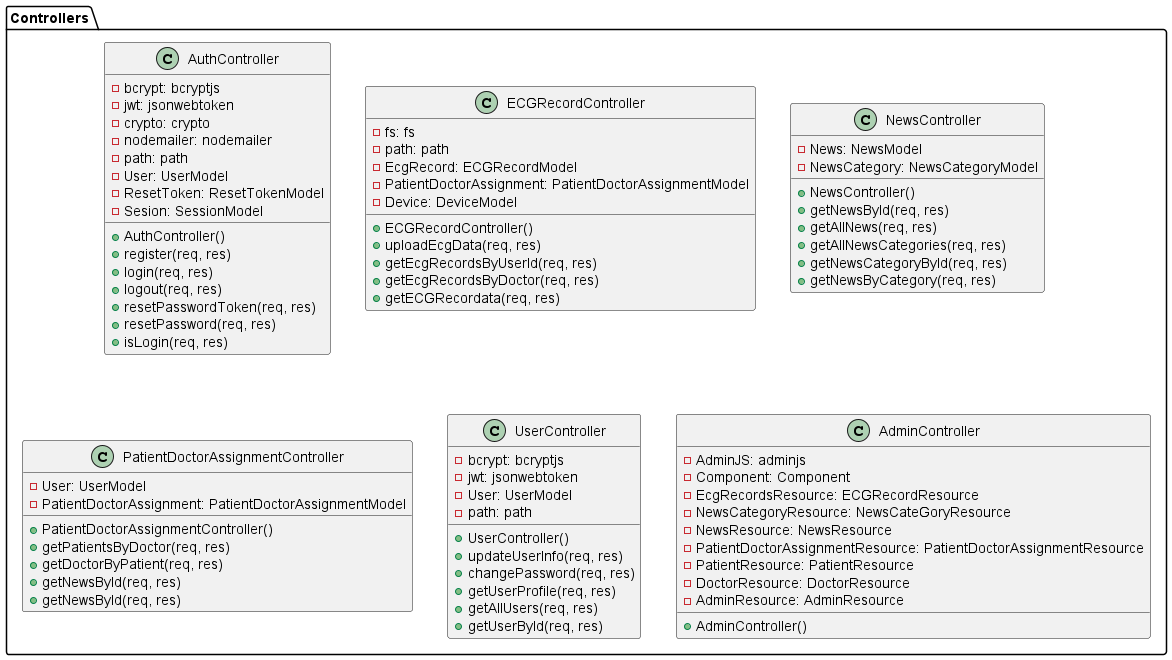
\includegraphics[width=15cm,height=12cm]{Images/server/class/class_controller.png}
  \caption[Sơ đồ lớp]{\bfseries \fontsize{12pt}{0pt}\selectfont Sơ đồ lớp}
  \label{hinh2} %đặt tên cho ảnh
\end{figure}



\begin{figure}[H]
  \centering
  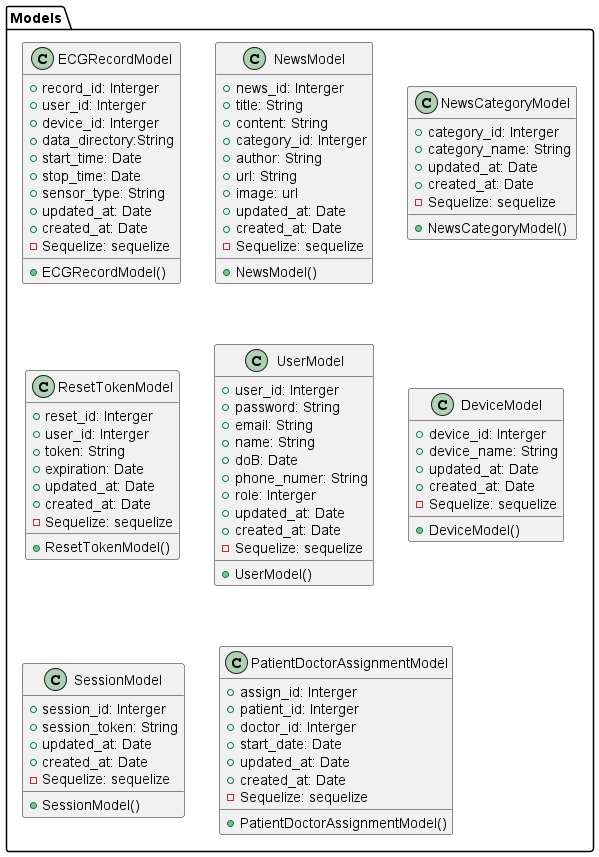
\includegraphics[width=15cm,height=12cm]{Images/server/class/class_model.png}
  \caption[Sơ đồ lớp]{\bfseries \fontsize{12pt}{0pt}\selectfont Sơ đồ lớp}
  \label{hinh2} %đặt tên cho ảnh
\end{figure}


\begin{figure}[H]
  \centering
  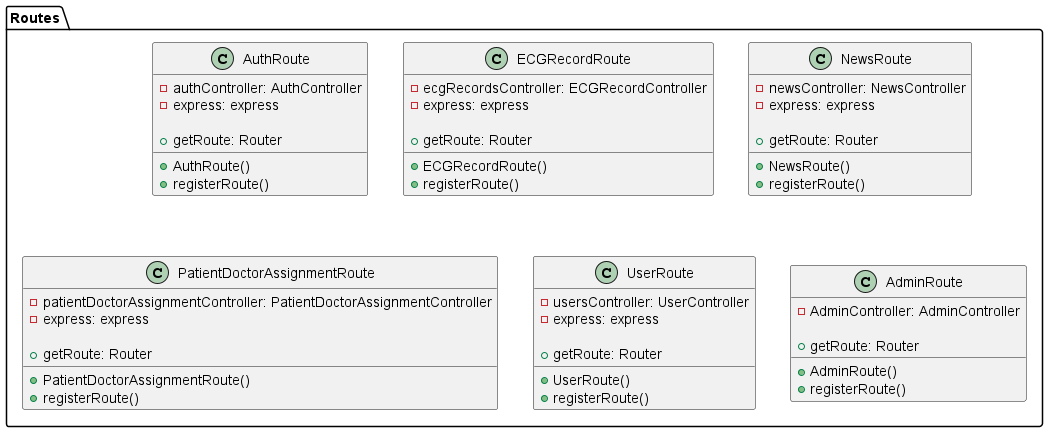
\includegraphics[width=15cm,height=12cm]{Images/server/class/class_route.png}
  \caption[Sơ đồ lớp]{\bfseries \fontsize{12pt}{0pt}\selectfont Sơ đồ lớp}
  \label{hinh2} %đặt tên cho ảnh
\end{figure}


\begin{figure}[H]
  \centering
  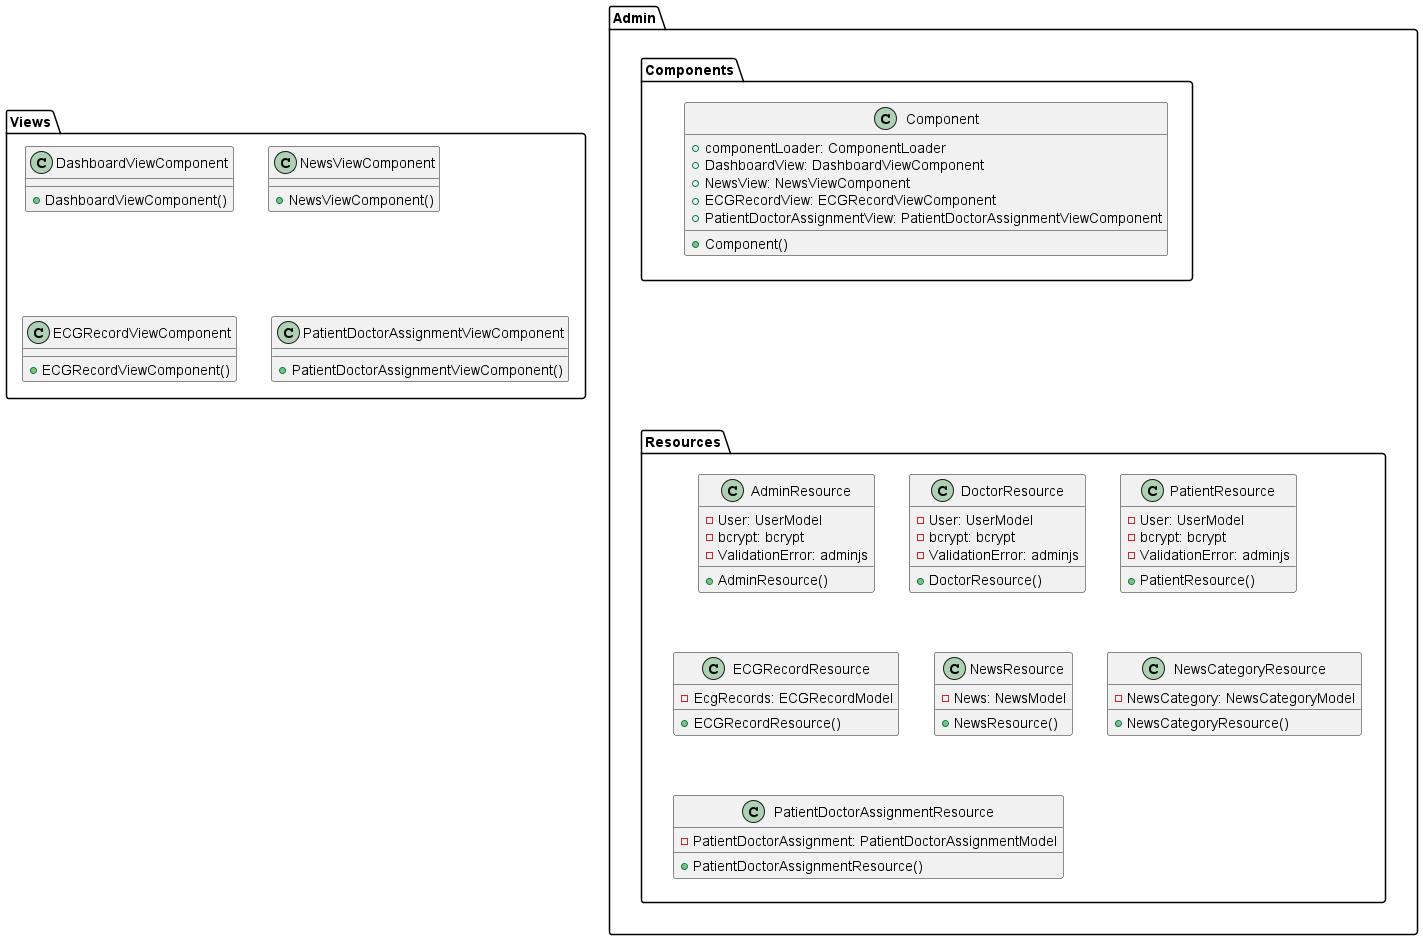
\includegraphics[width=15cm,height=12cm]{Images/server/class/class_admin.png}
  \caption[Sơ đồ lớp]{\bfseries \fontsize{12pt}{0pt}\selectfont Sơ đồ lớp}
  \label{hinh2} %đặt tên cho ảnh
\end{figure}


\item Mối quan hệ

\begin{figure}[H]
  \centering
  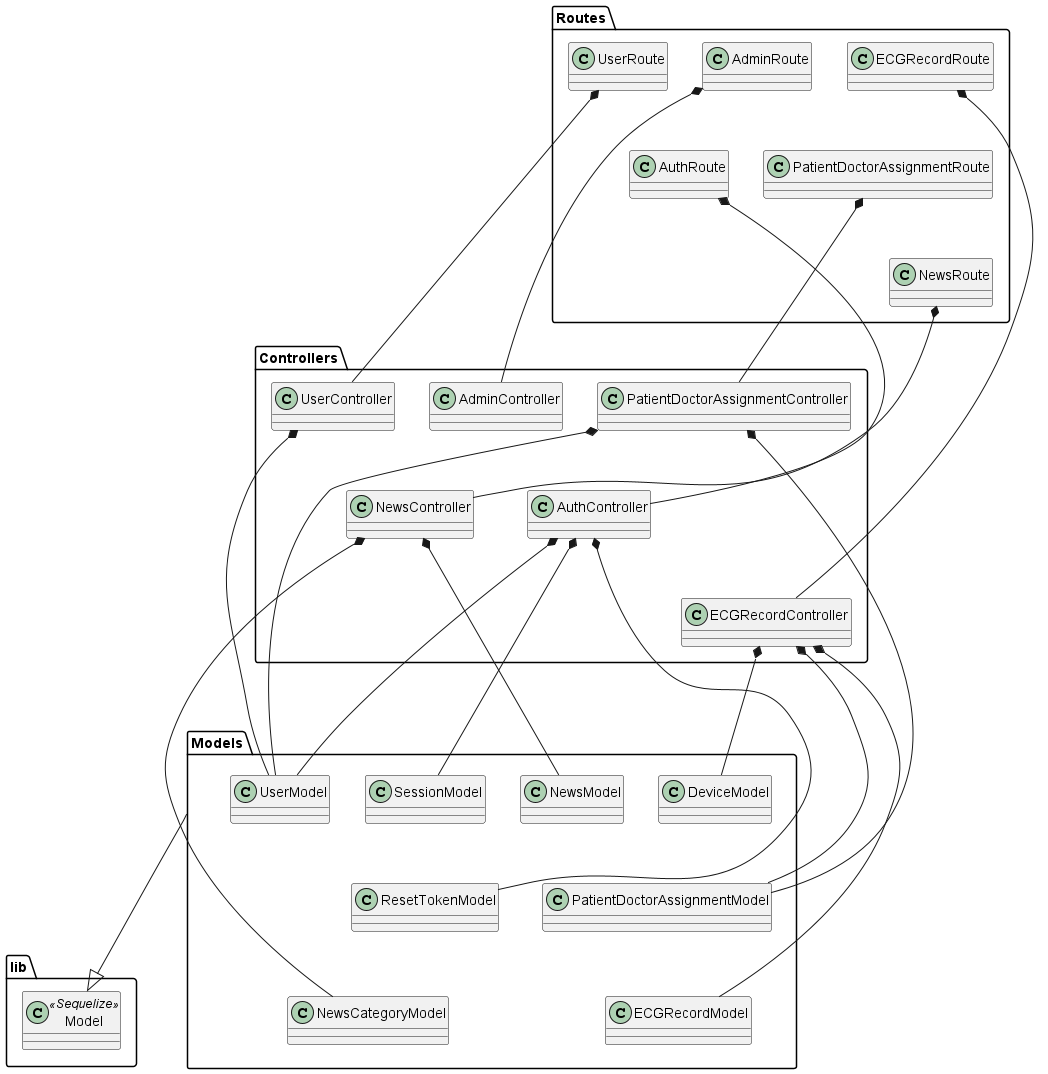
\includegraphics[width=15cm,height=12cm]{Images/server/class/class_relation.png}
  \caption[Sơ đồ lớp]{\bfseries \fontsize{12pt}{0pt}\selectfont Sơ đồ lớp}
  \label{hinh2} %đặt tên cho ảnh
\end{figure}


\begin{figure}[H]
  \centering
  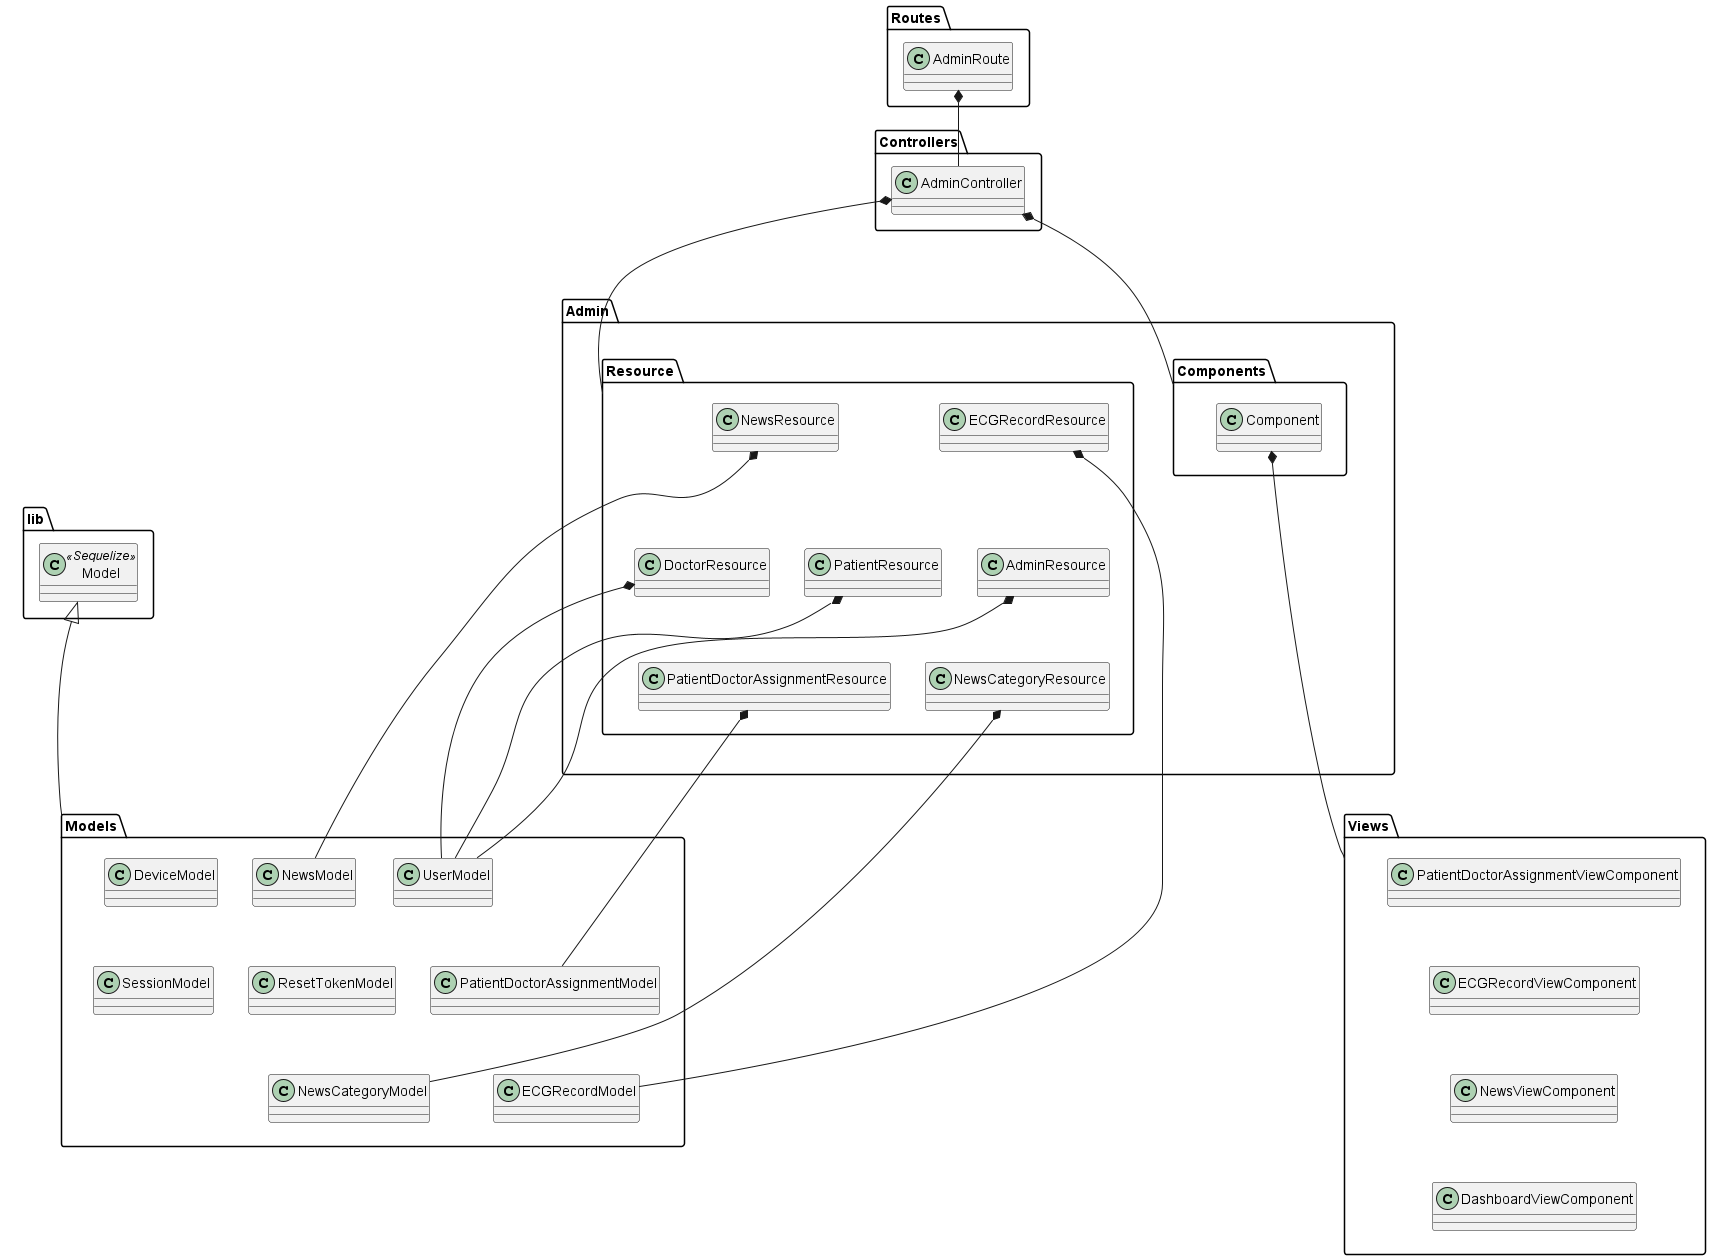
\includegraphics[width=15cm,height=12cm]{Images/server/class/class_admin_relation.png}
  \caption[Sơ đồ lớp]{\bfseries \fontsize{12pt}{0pt}\selectfont Sơ đồ lớp}
  \label{hinh2} %đặt tên cho ảnh
\end{figure}

\end{enumerate}


\subsubsection{Sơ đồ tuần tự}

\begin{figure}[H]
  \centering
  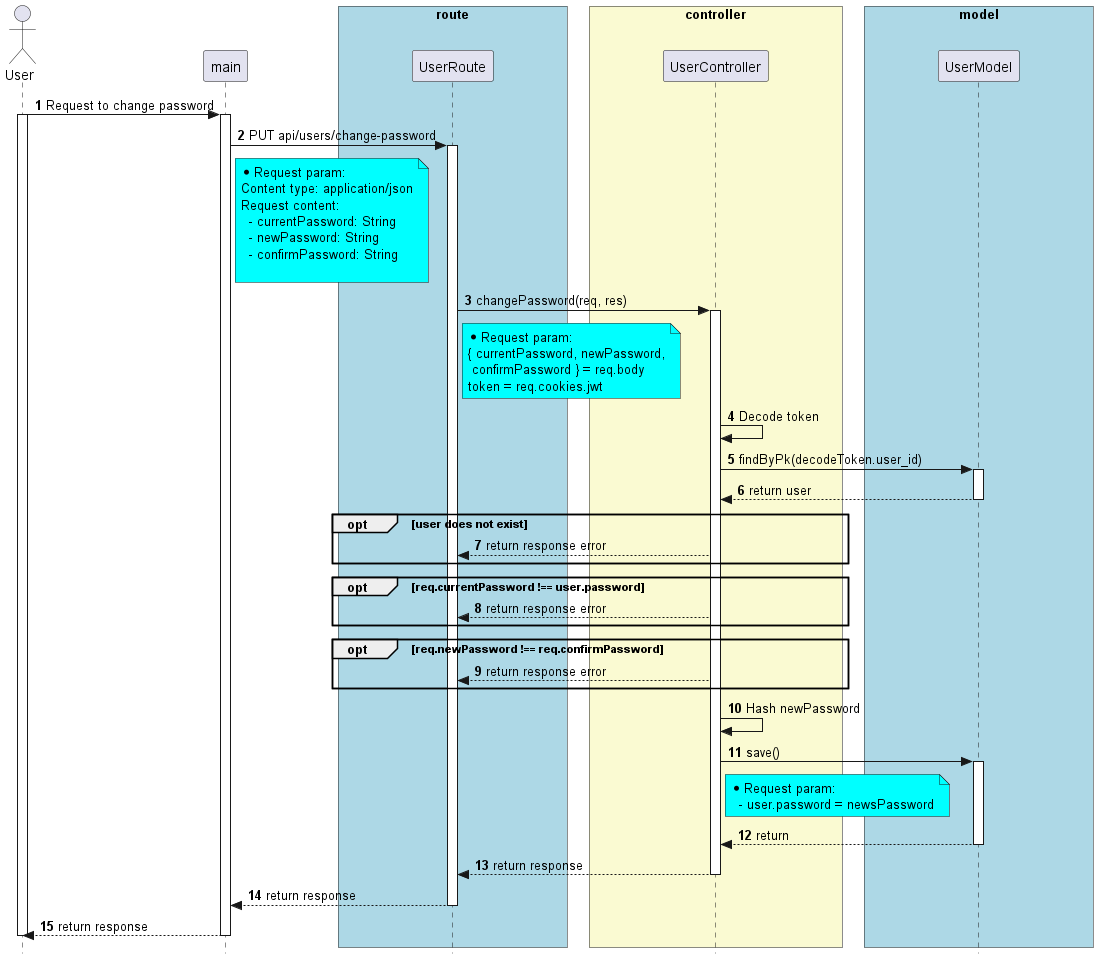
\includegraphics[width=16cm,height=9cm]{Images/server/sequence/server/changePassword.png}
  \caption[Sơ đồ tuần tự ]{\bfseries \fontsize{12pt}{0pt}
  \selectfont Sơ đồ tuần }
  \label{hinh21} %đặt tên cho ảnh
\end{figure}


\begin{figure}[H]
  \centering
  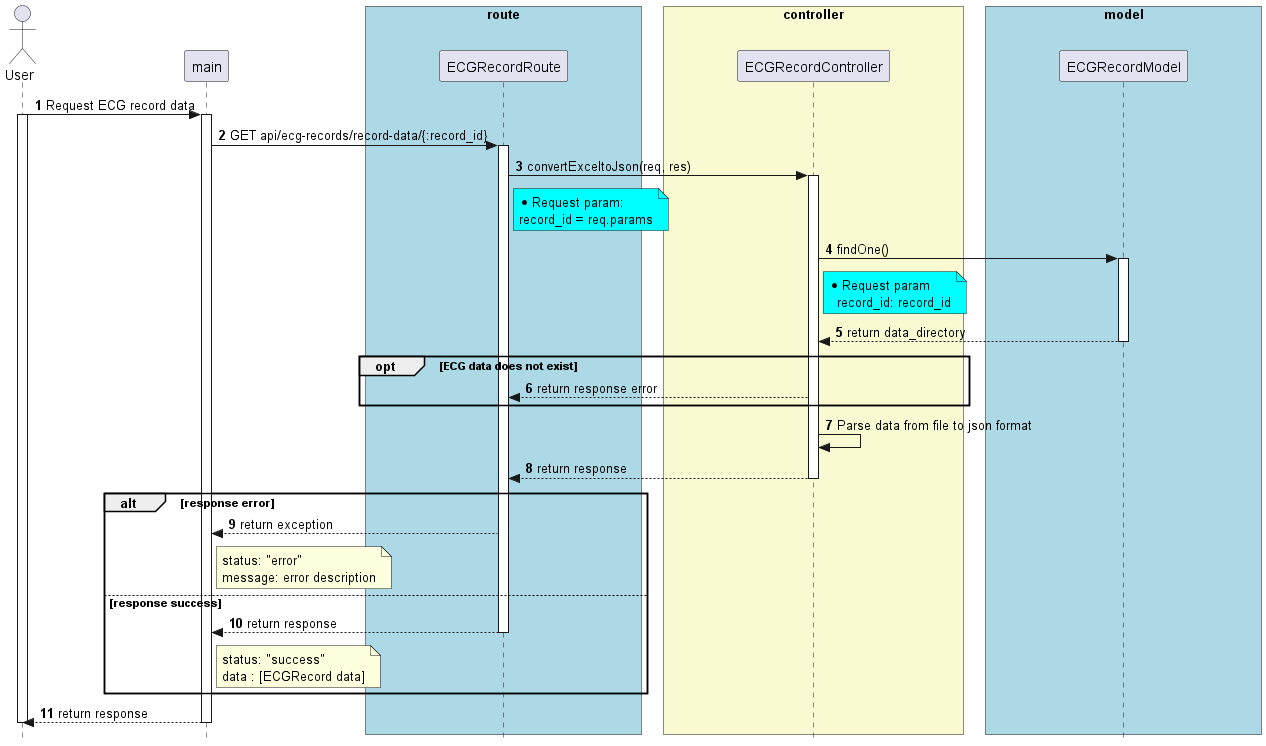
\includegraphics[width=16cm,height=9cm]{Images/server/sequence/server/convertExceltoJson.png}
  \caption[Sơ đồ tuần tự ]{\bfseries \fontsize{12pt}{0pt}
  \selectfont Sơ đồ tuần }
  \label{hinh21} %đặt tên cho ảnh
\end{figure}


\begin{figure}[H]
  \centering
  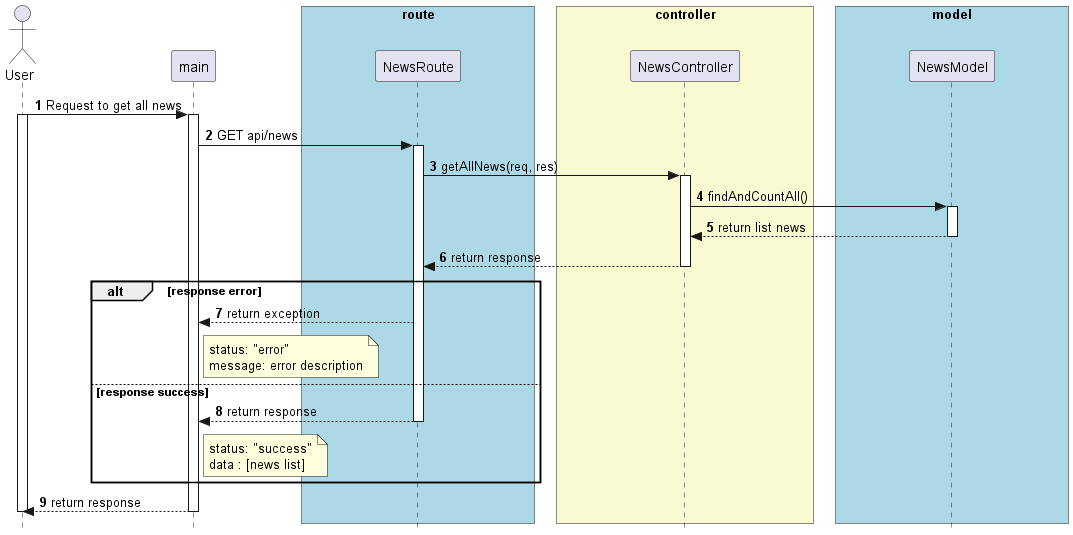
\includegraphics[width=16cm,height=9cm]{Images/server/sequence/server/getAllNews.png}
  \caption[Sơ đồ tuần tự ]{\bfseries \fontsize{12pt}{0pt}
  \selectfont Sơ đồ tuần }
  \label{hinh21} %đặt tên cho ảnh
\end{figure}

\begin{figure}[H]
  \centering
  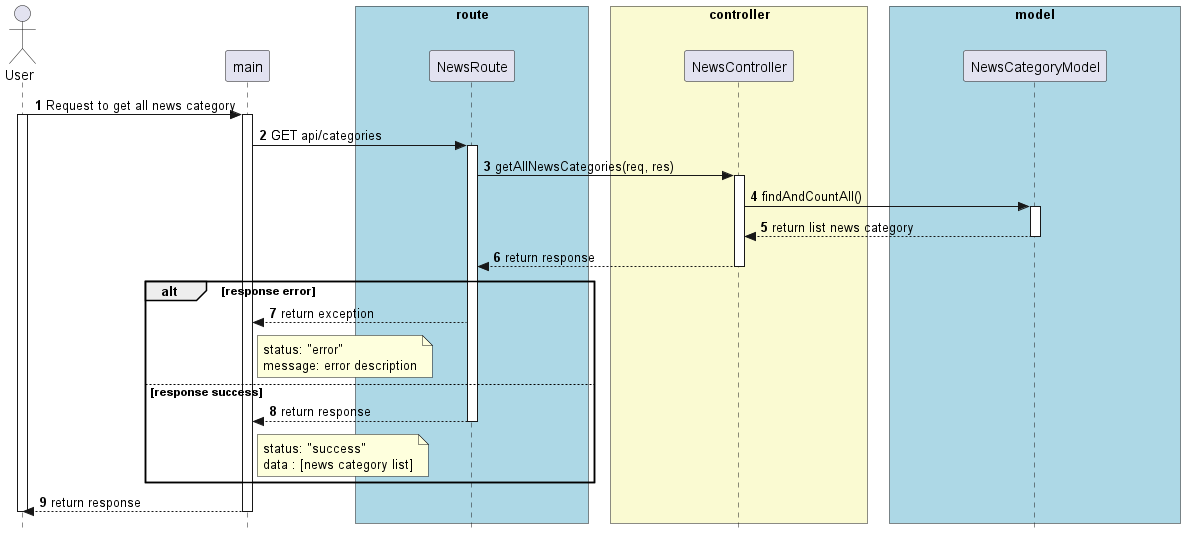
\includegraphics[width=16cm,height=9cm]{Images/server/sequence/server/getAllNewsCategories.png}
  \caption[Sơ đồ tuần tự ]{\bfseries \fontsize{12pt}{0pt}
  \selectfont Sơ đồ tuần }
  \label{hinh21} %đặt tên cho ảnh
\end{figure}


\begin{figure}[H]
  \centering
  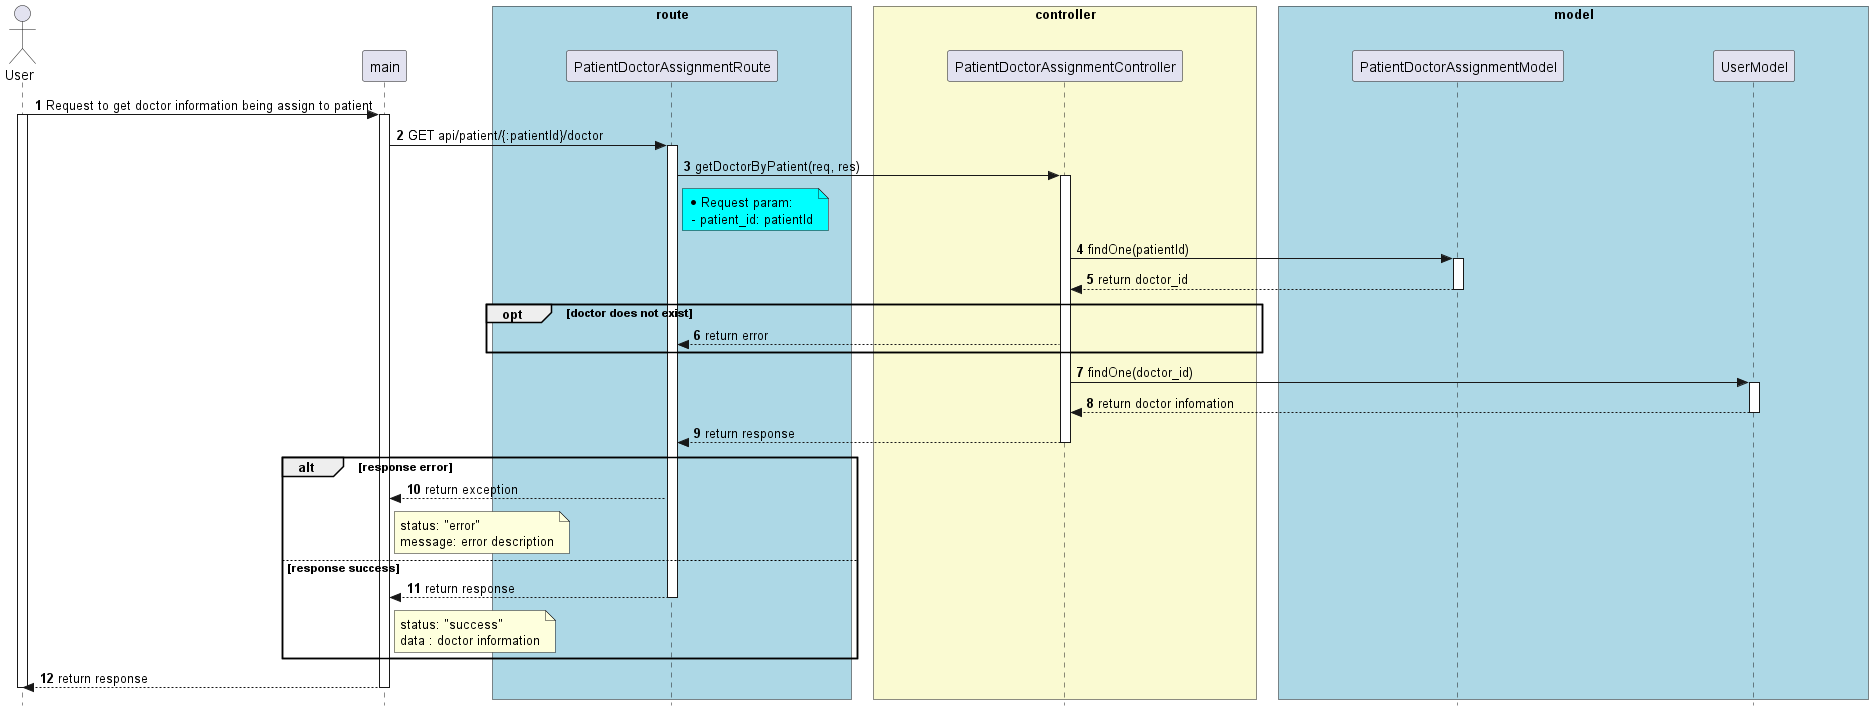
\includegraphics[width=16cm,height=9cm]{Images/server/sequence/server/getDoctorByPatient.png}
  \caption[Sơ đồ tuần tự ]{\bfseries \fontsize{12pt}{0pt}
  \selectfont Sơ đồ tuần }
  \label{hinh21} %đặt tên cho ảnh
\end{figure}


\begin{figure}[H]
  \centering
  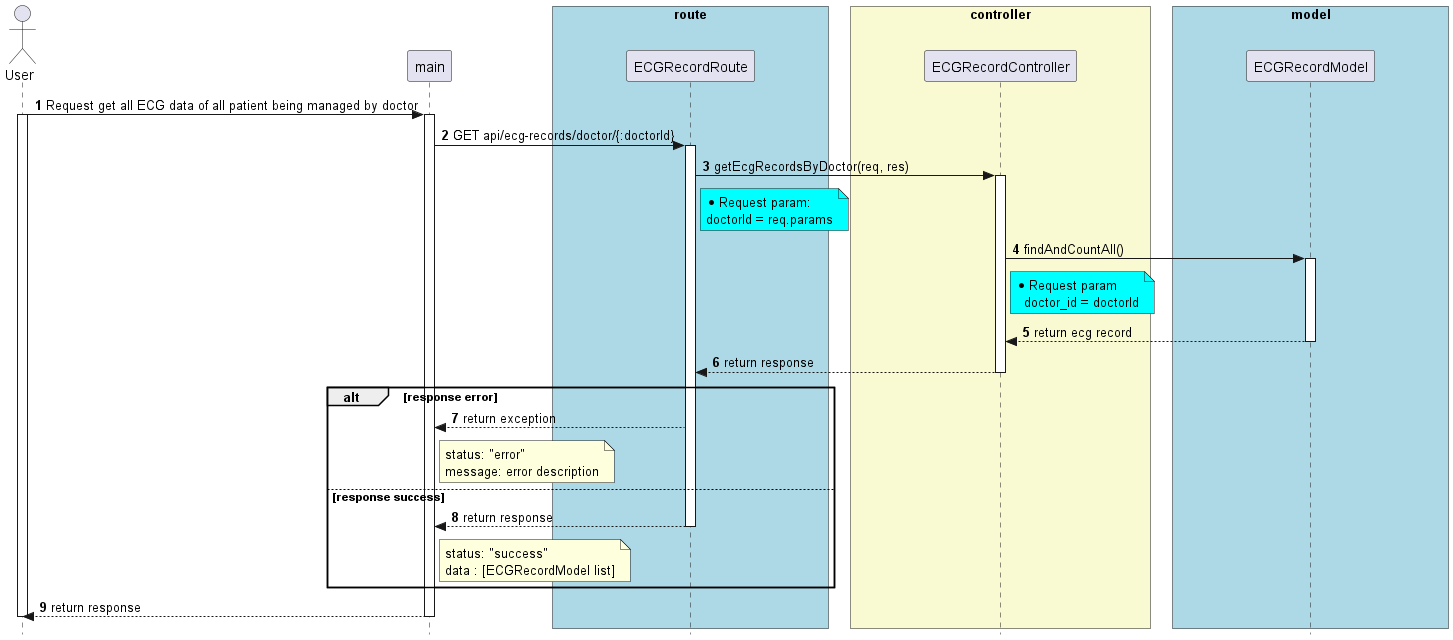
\includegraphics[width=16cm,height=9cm]{Images/server/sequence/server/getEcgRecordsByDoctor.png}
  \caption[Sơ đồ tuần tự ]{\bfseries \fontsize{12pt}{0pt}
  \selectfont Sơ đồ tuần }
  \label{hinh21} %đặt tên cho ảnh
\end{figure}


\begin{figure}[H]
  \centering
  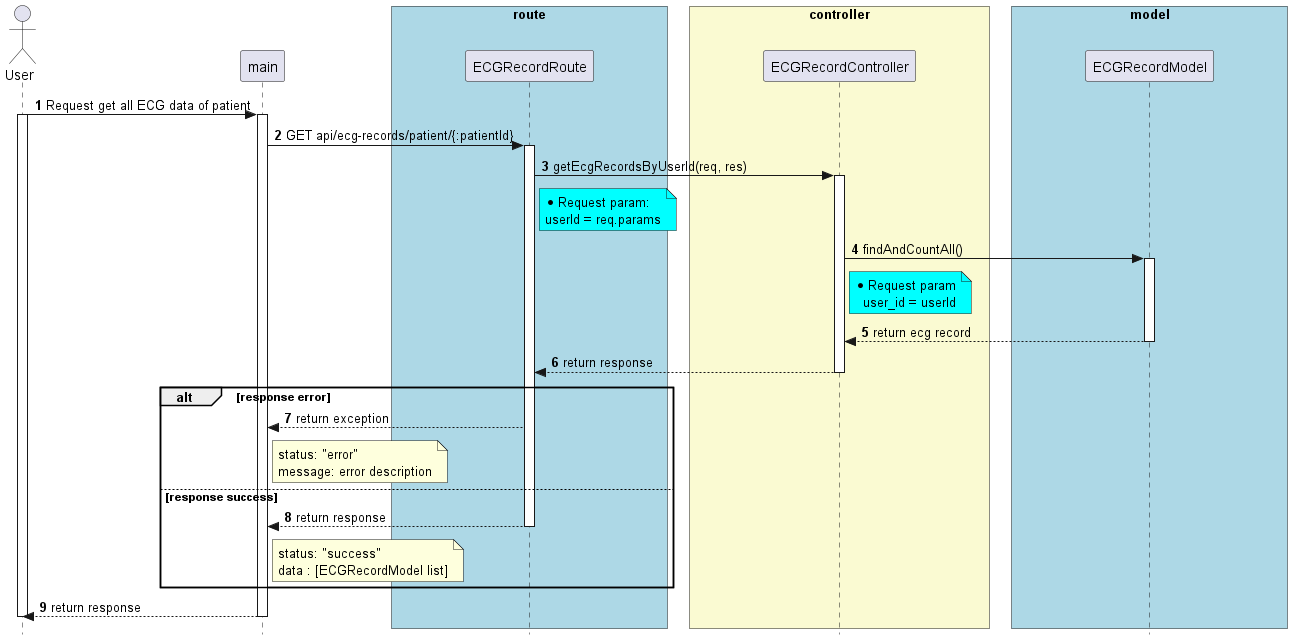
\includegraphics[width=16cm,height=9cm]{Images/server/sequence/server/getEcgRecordsByUserId.png}
  \caption[Sơ đồ tuần tự ]{\bfseries \fontsize{12pt}{0pt}
  \selectfont Sơ đồ tuần }
  \label{hinh21} %đặt tên cho ảnh
\end{figure}


\begin{figure}[H]
  \centering
  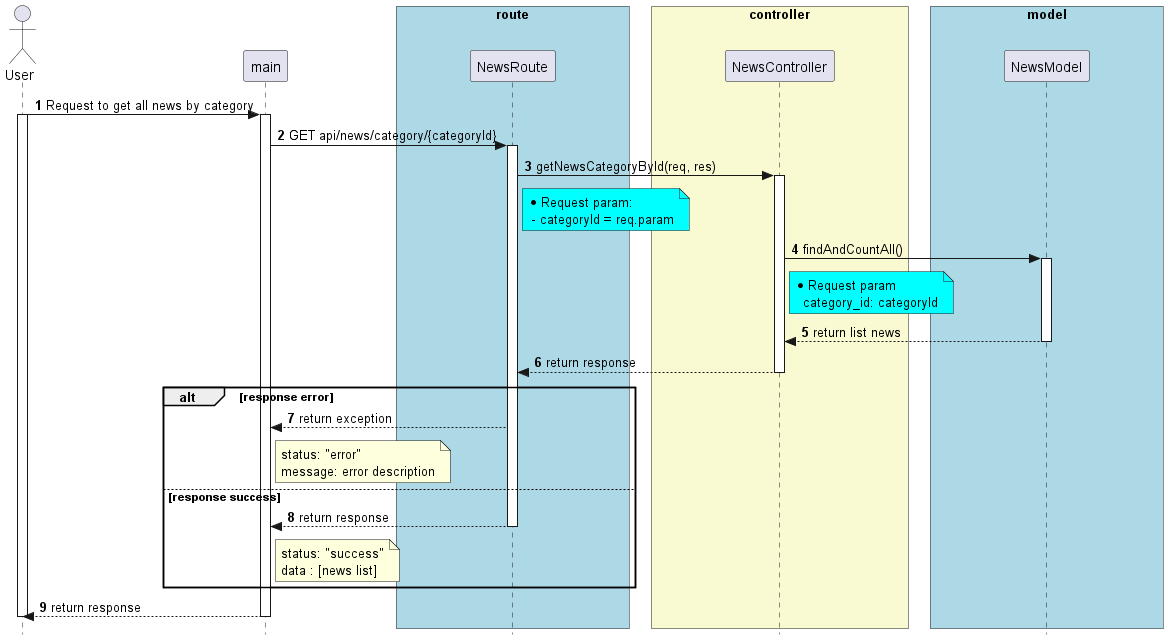
\includegraphics[width=16cm,height=9cm]{Images/server/sequence/server/getNewsByCategory.png}
  \caption[Sơ đồ tuần tự ]{\bfseries \fontsize{12pt}{0pt}
  \selectfont Sơ đồ tuần }
  \label{hinh21} %đặt tên cho ảnh
\end{figure}


\begin{figure}[H]
  \centering
  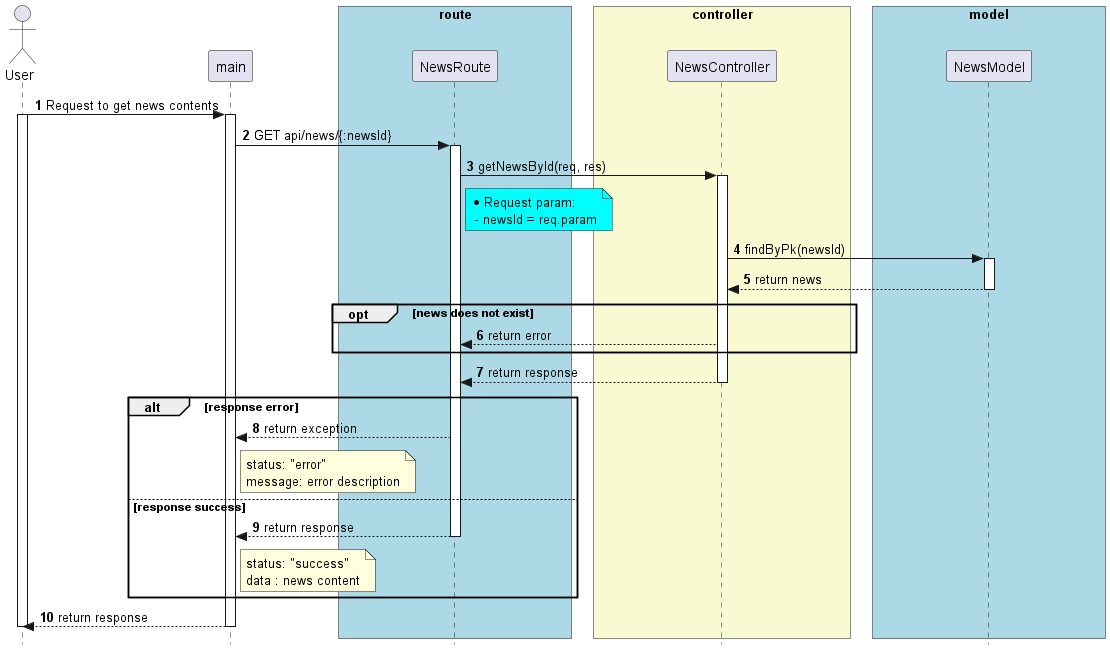
\includegraphics[width=16cm,height=9cm]{Images/server/sequence/server/getNewsById.png}
  \caption[Sơ đồ tuần tự ]{\bfseries \fontsize{12pt}{0pt}
  \selectfont Sơ đồ tuần }
  \label{hinh21} %đặt tên cho ảnh
\end{figure}


\begin{figure}[H]
  \centering
  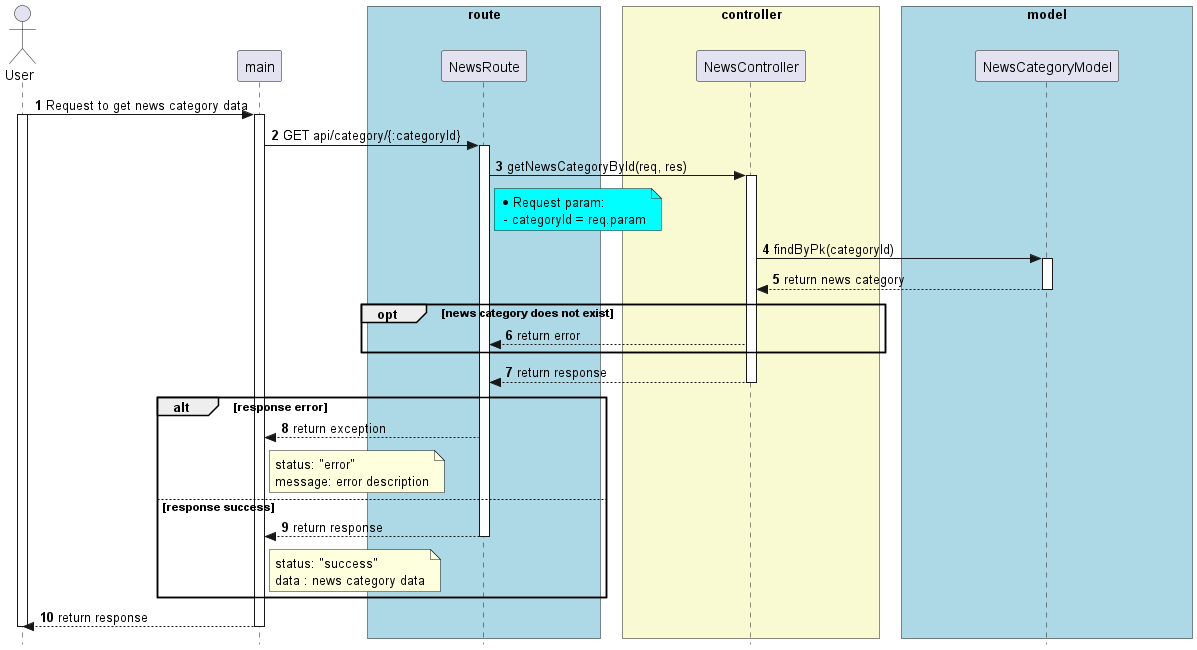
\includegraphics[width=16cm,height=9cm]{Images/server/sequence/server/getNewsCategoryById.png}
  \caption[Sơ đồ tuần tự ]{\bfseries \fontsize{12pt}{0pt}
  \selectfont Sơ đồ tuần }
  \label{hinh21} %đặt tên cho ảnh
\end{figure}

\begin{figure}[H]
  \centering
  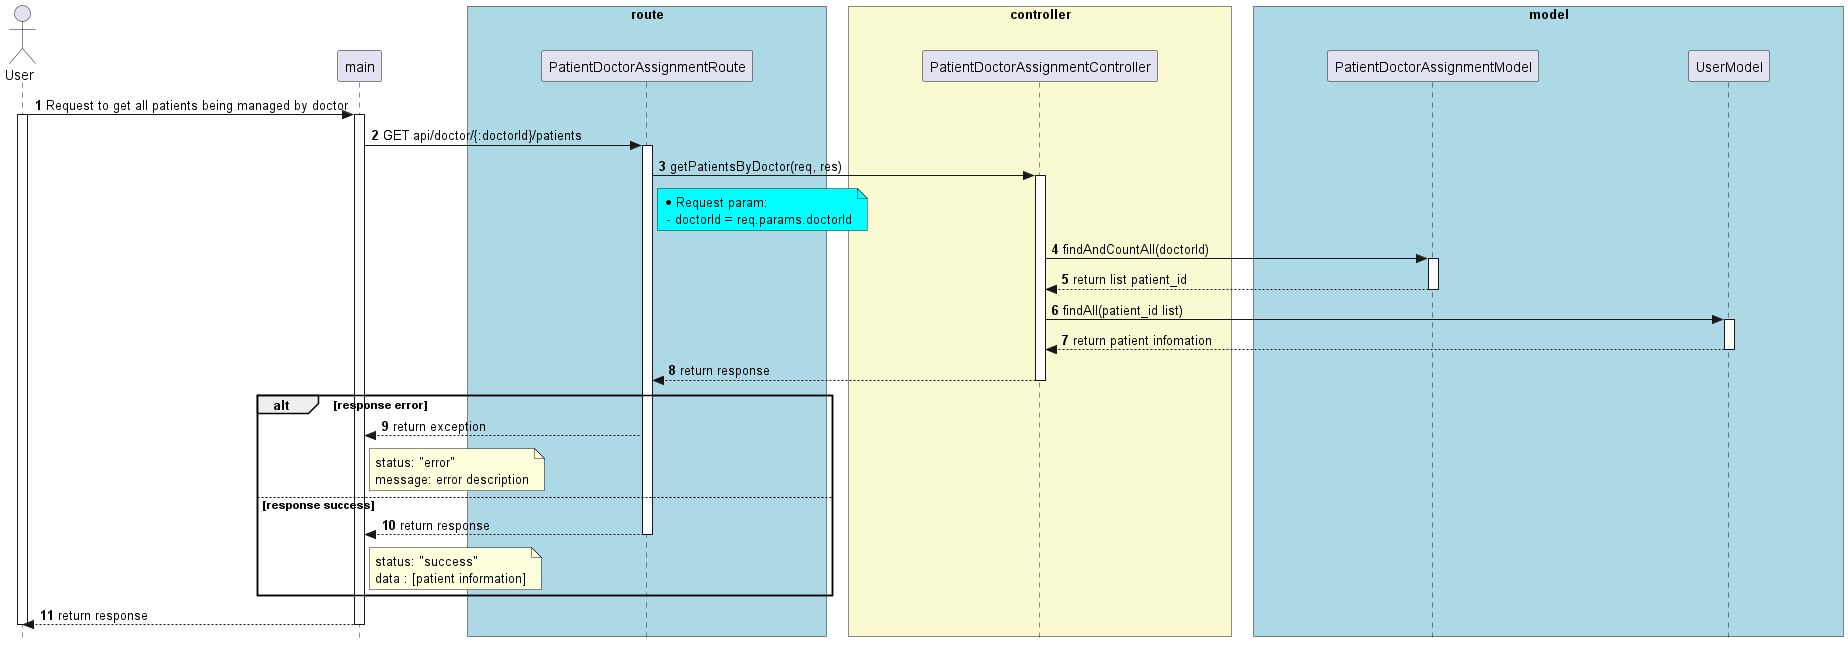
\includegraphics[width=16cm,height=9cm]{Images/server/sequence/server/getPatientsByDoctor.png}
  \caption[Sơ đồ tuần tự ]{\bfseries \fontsize{12pt}{0pt}
  \selectfont Sơ đồ tuần }
  \label{hinh21} %đặt tên cho ảnh
\end{figure}

\begin{figure}[H]
  \centering
  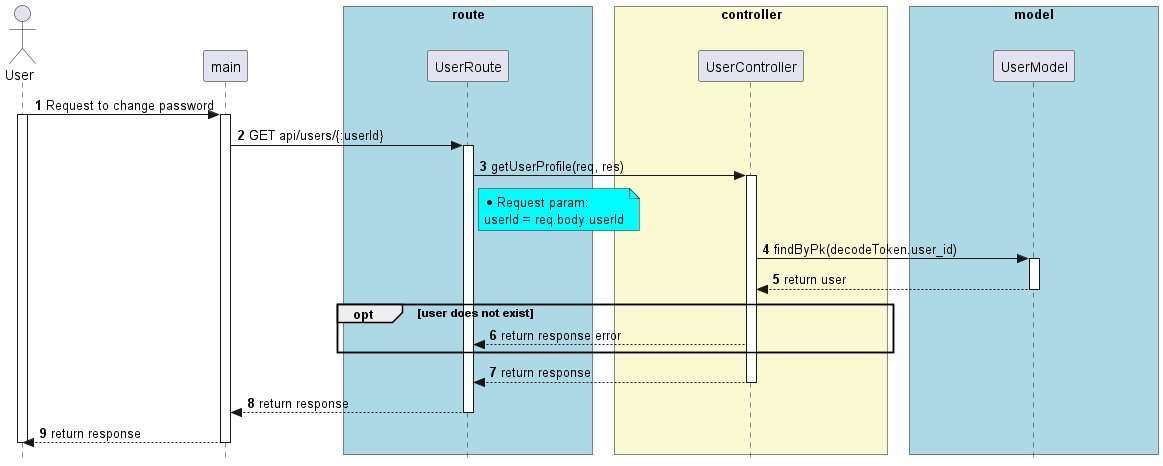
\includegraphics[width=16cm,height=9cm]{Images/server/sequence/server/getUserById.png}
  \caption[Sơ đồ tuần tự ]{\bfseries \fontsize{12pt}{0pt}
  \selectfont Sơ đồ tuần }
  \label{hinh21} %đặt tên cho ảnh
\end{figure}

\begin{figure}[H]
  \centering
  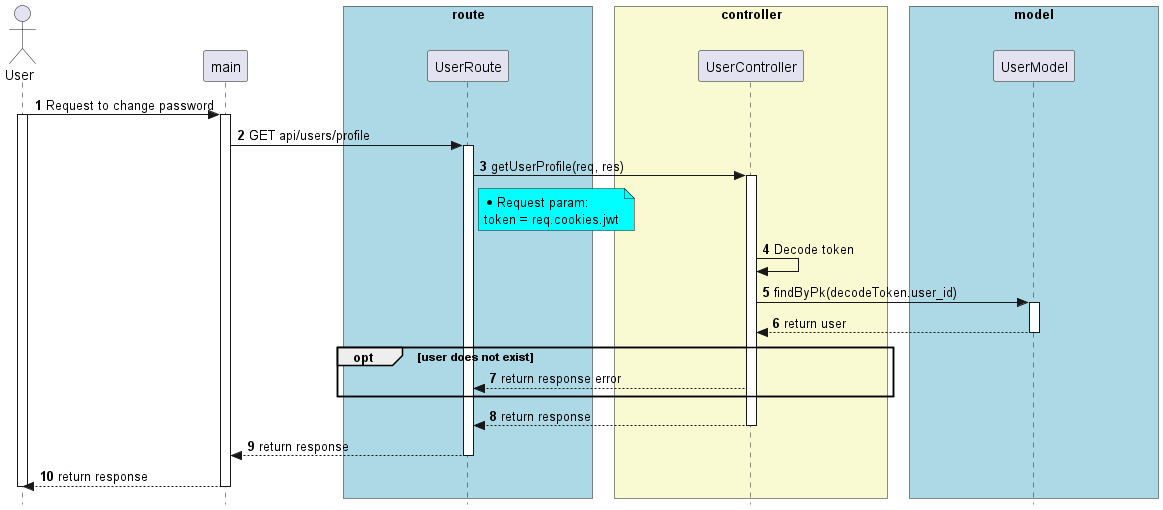
\includegraphics[width=16cm,height=9cm]{Images/server/sequence/server/getUserProfile.png}
  \caption[Sơ đồ tuần tự ]{\bfseries \fontsize{12pt}{0pt}
  \selectfont Sơ đồ tuần }
  \label{hinh21} %đặt tên cho ảnh
\end{figure}

\begin{figure}[H]
  \centering
  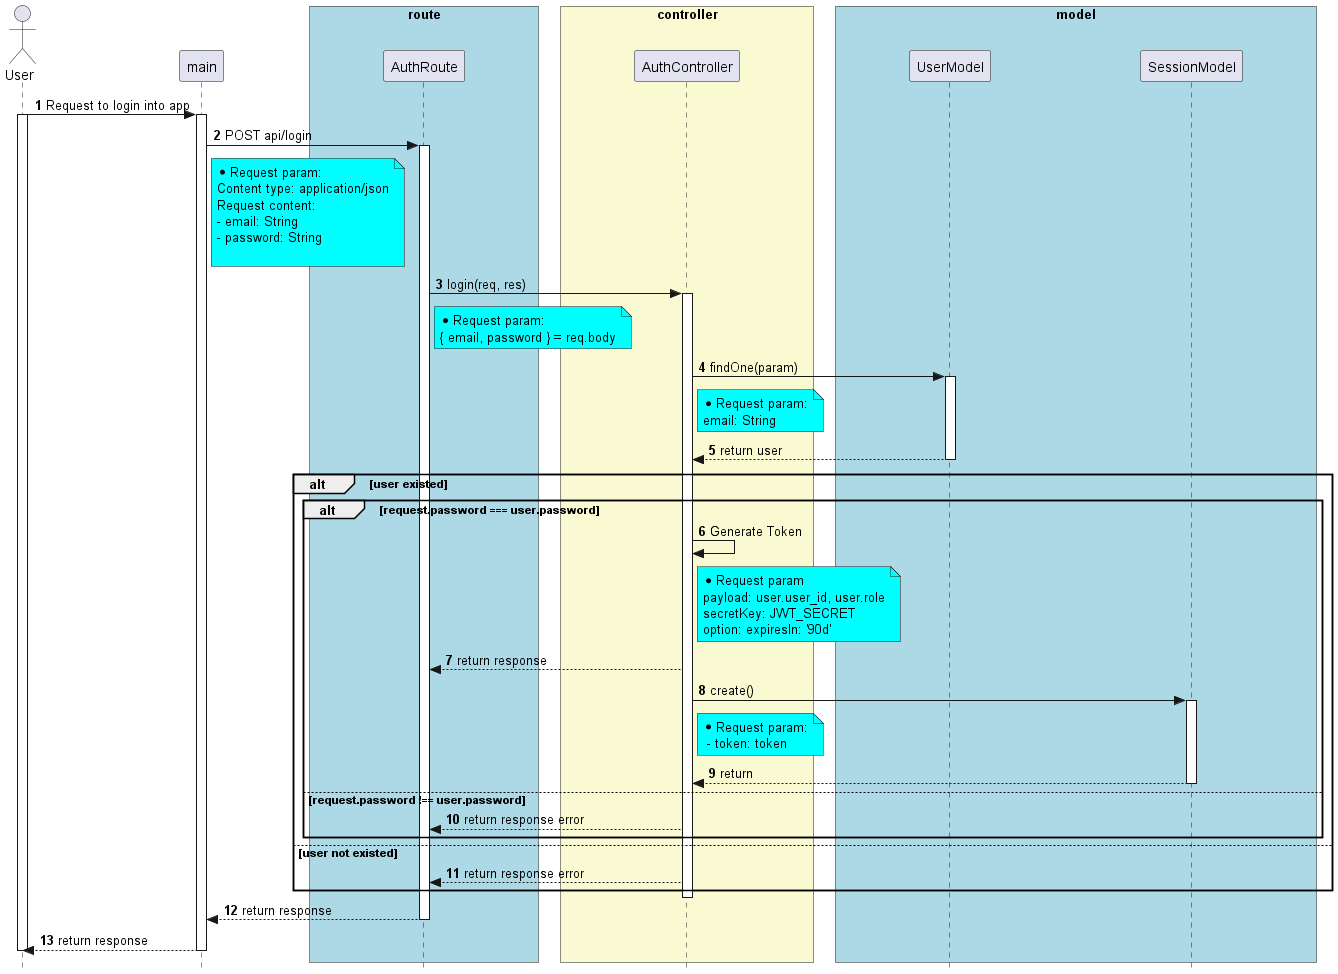
\includegraphics[width=16cm,height=9cm]{Images/server/sequence/server/login.png}
  \caption[Sơ đồ tuần tự ]{\bfseries \fontsize{12pt}{0pt}
  \selectfont Sơ đồ tuần }
  \label{hinh21} %đặt tên cho ảnh
\end{figure}

\begin{figure}[H]
  \centering
  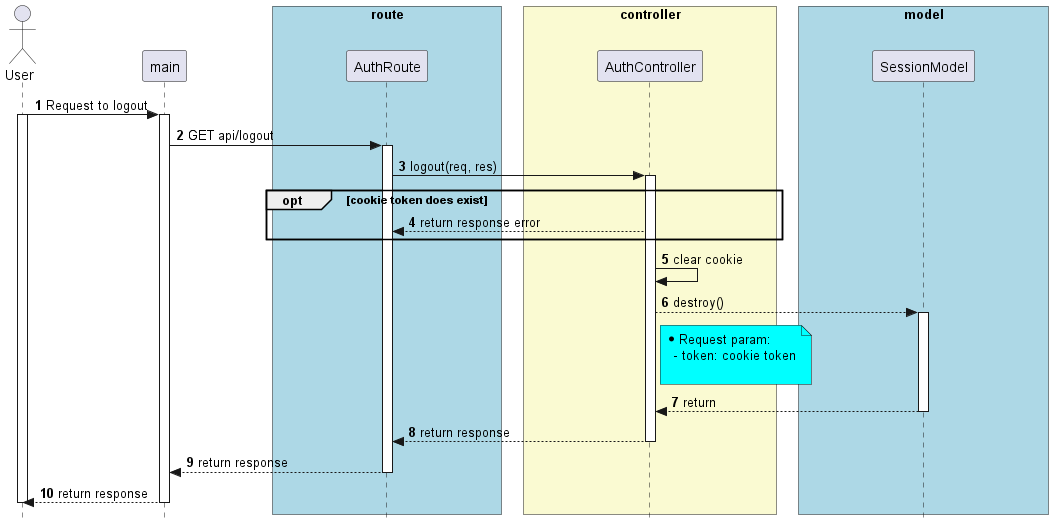
\includegraphics[width=16cm,height=9cm]{Images/server/sequence/server/logout.png}
  \caption[Sơ đồ tuần tự ]{\bfseries \fontsize{12pt}{0pt}
  \selectfont Sơ đồ tuần }
  \label{hinh21} %đặt tên cho ảnh
\end{figure}


\begin{figure}[H]
  \centering
  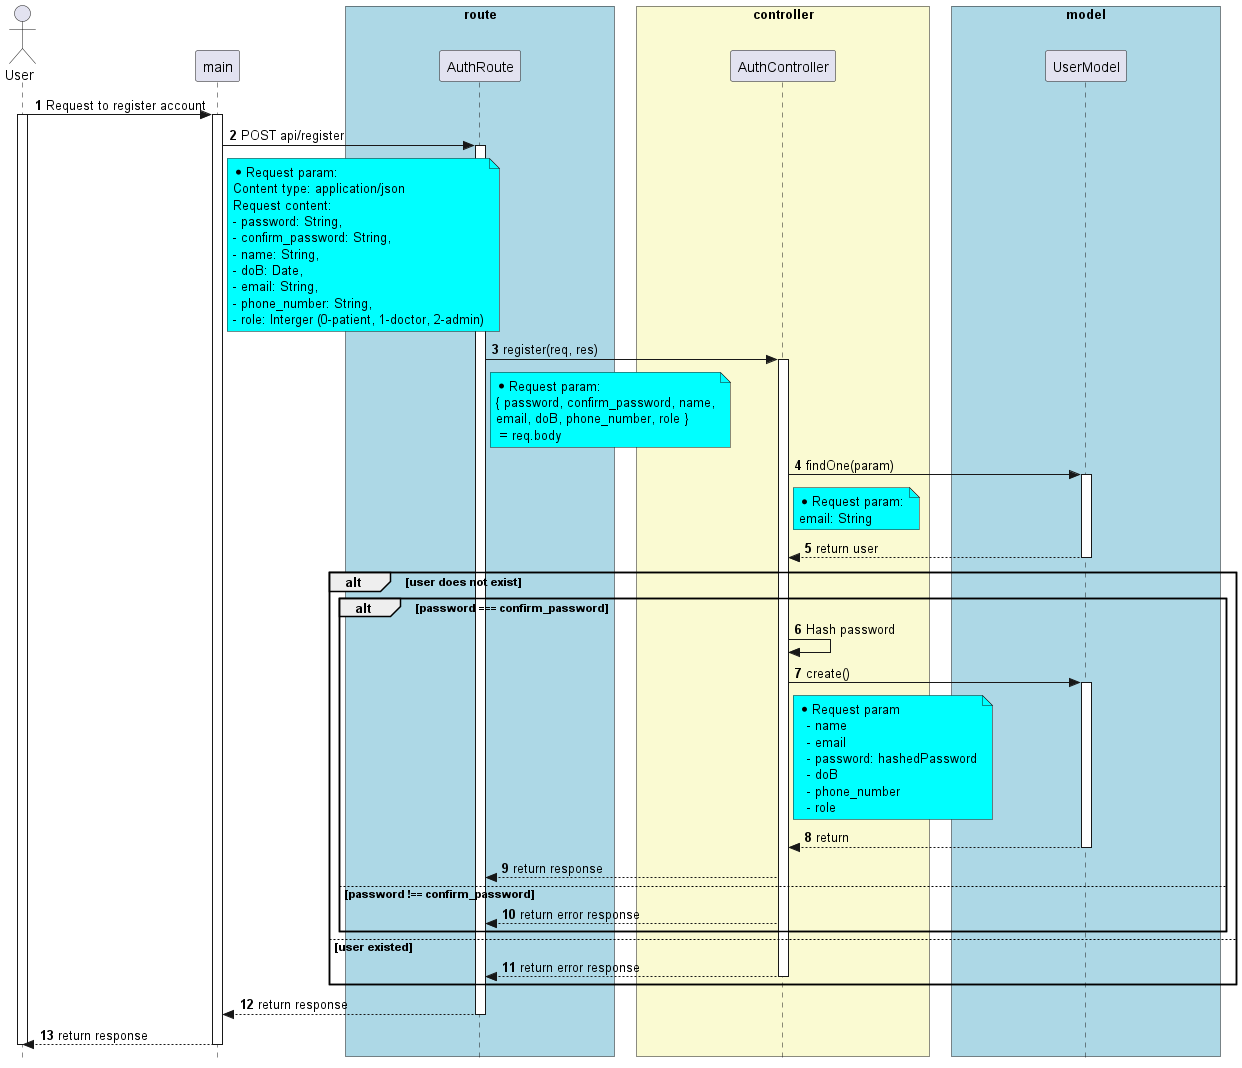
\includegraphics[width=16cm,height=9cm]{Images/server/sequence/server/register.png}
  \caption[Sơ đồ tuần tự ]{\bfseries \fontsize{12pt}{0pt}
  \selectfont Sơ đồ tuần }
  \label{hinh21} %đặt tên cho ảnh
\end{figure}

\begin{figure}[H]
  \centering
  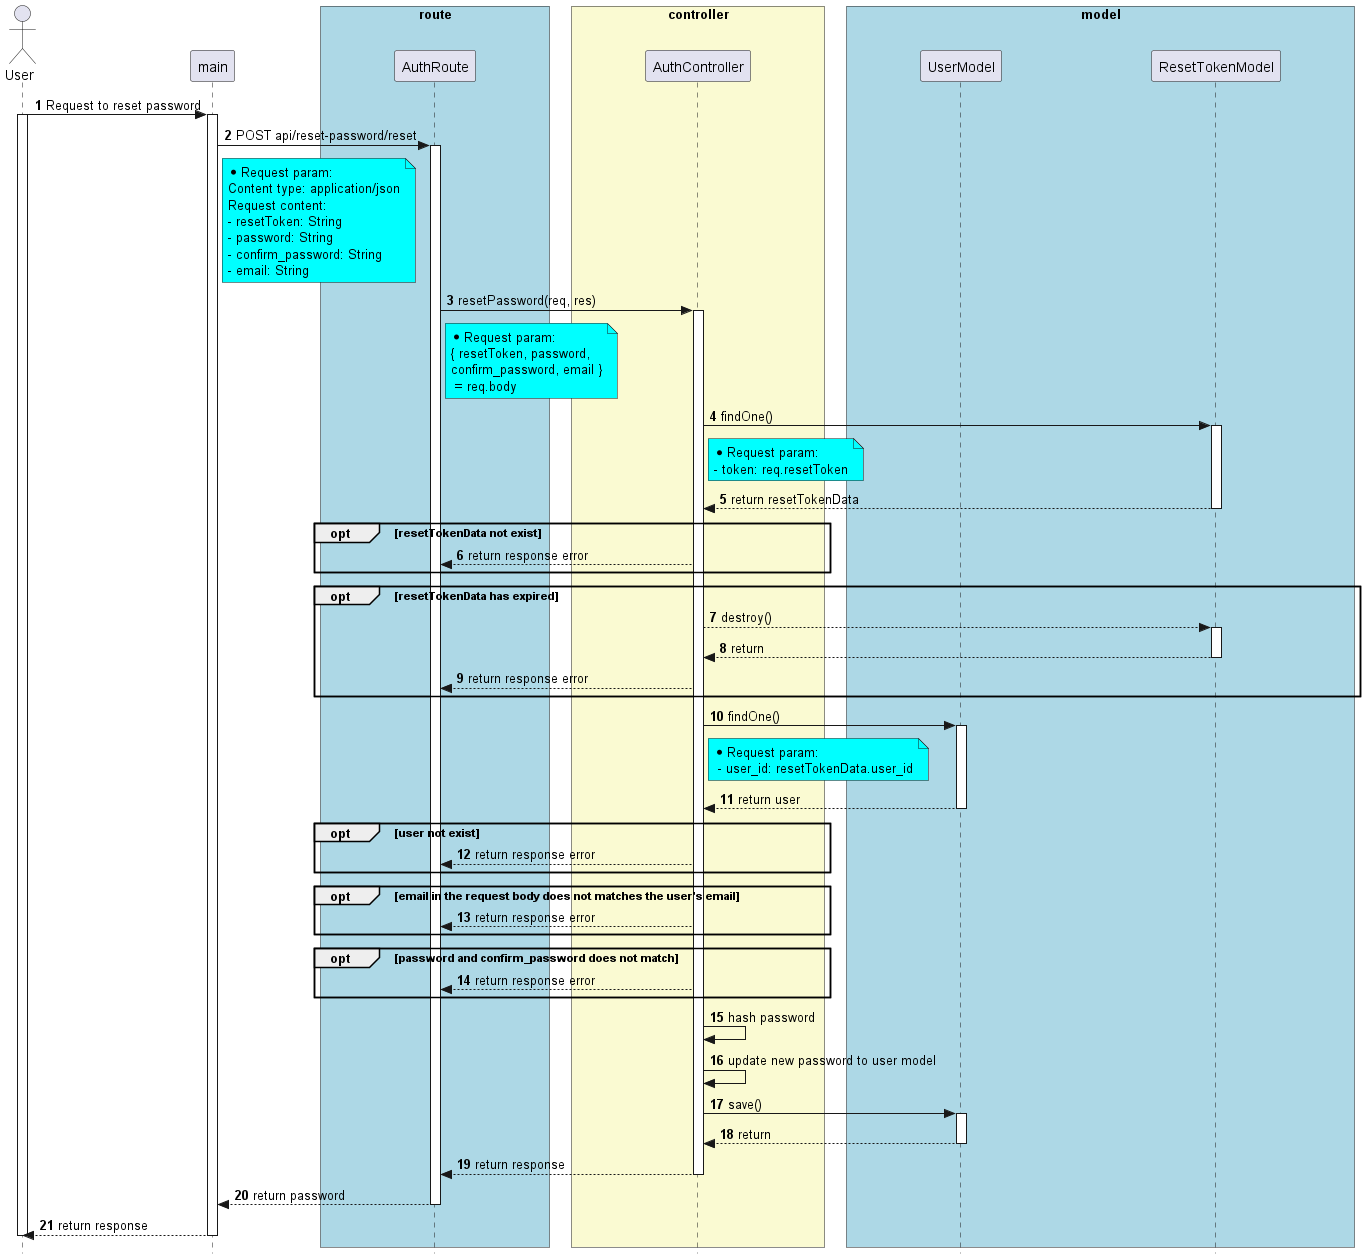
\includegraphics[width=16cm,height=9cm]{Images/server/sequence/server/resetPassword.png}
  \caption[Sơ đồ tuần tự ]{\bfseries \fontsize{12pt}{0pt}
  \selectfont Sơ đồ tuần }
  \label{hinh21} %đặt tên cho ảnh
\end{figure}

\begin{figure}[H]
  \centering
  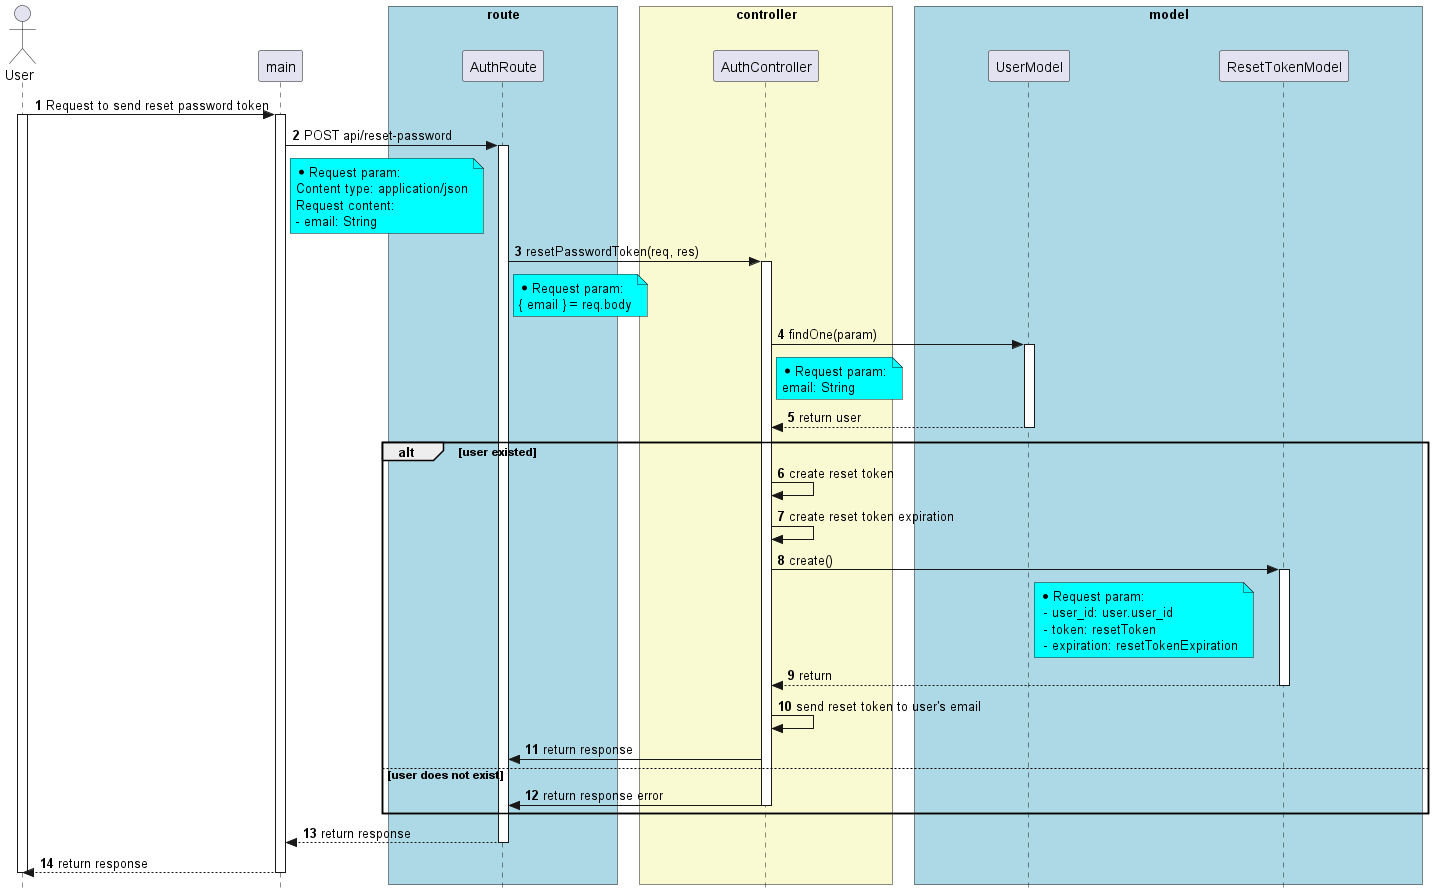
\includegraphics[width=16cm,height=9cm]{Images/server/sequence/server/resetPasswordToken.png}
  \caption[Sơ đồ tuần tự ]{\bfseries \fontsize{12pt}{0pt}
  \selectfont Sơ đồ tuần }
  \label{hinh21} %đặt tên cho ảnh
\end{figure}

\begin{figure}[H]
  \centering
  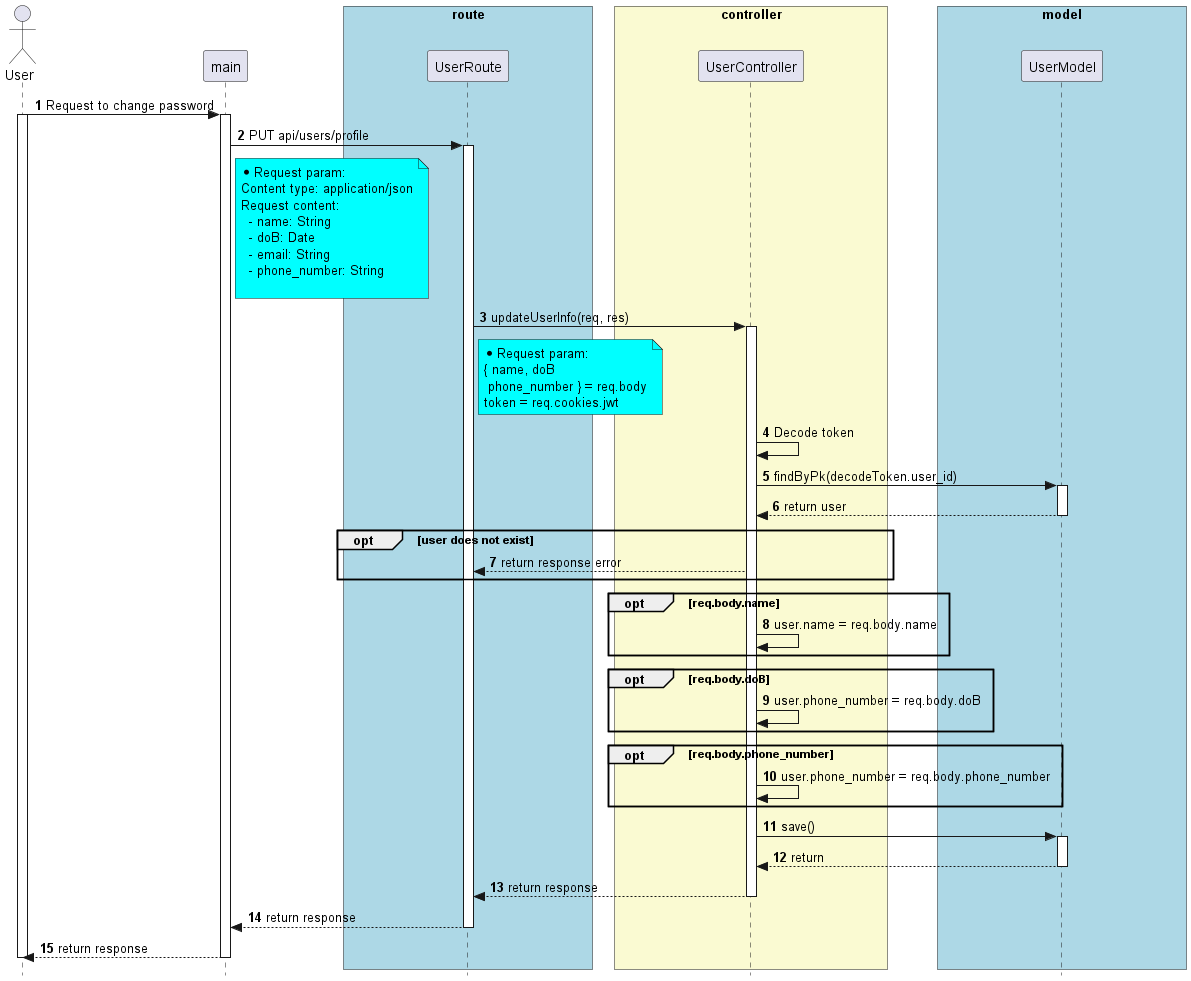
\includegraphics[width=16cm,height=9cm]{Images/server/sequence/server/updateUserInfo.png}
  \caption[Sơ đồ tuần tự ]{\bfseries \fontsize{12pt}{0pt}
  \selectfont Sơ đồ tuần }
  \label{hinh21} %đặt tên cho ảnh
\end{figure}



\begin{figure}[H]
  \centering
  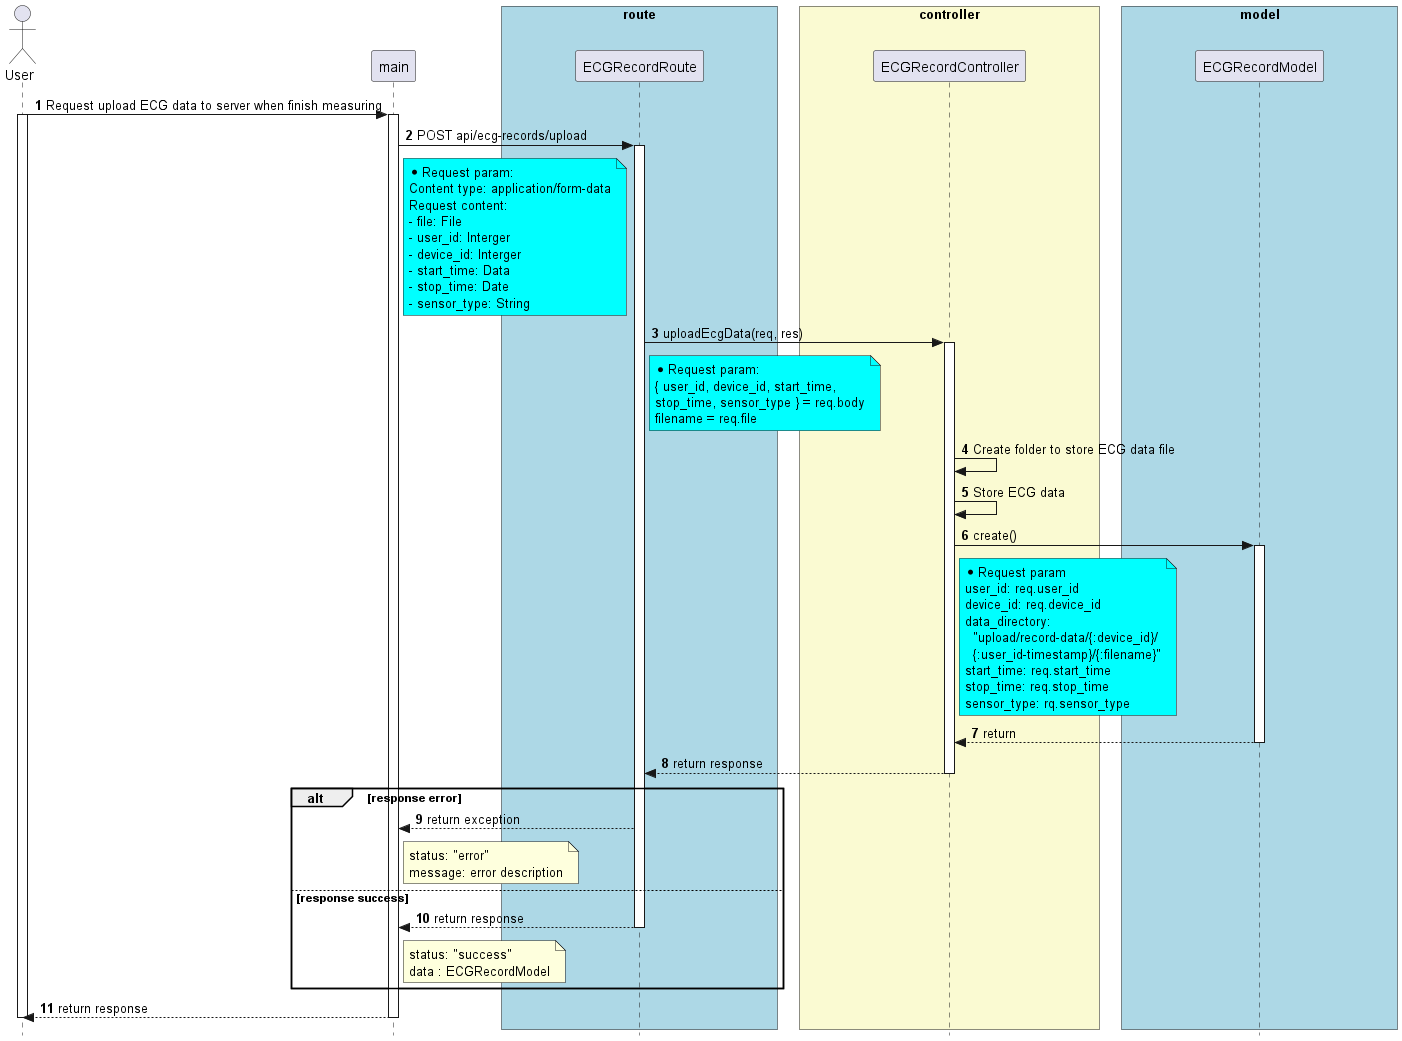
\includegraphics[width=16cm,height=9cm]{Images/server/sequence/server/uploadEcgData.png}
  \caption[Sơ đồ tuần tự ]{\bfseries \fontsize{12pt}{0pt}
  \selectfont Sơ đồ tuần }
  \label{hinh21} %đặt tên cho ảnh
\end{figure}


\begin{figure}[H]
  \centering
  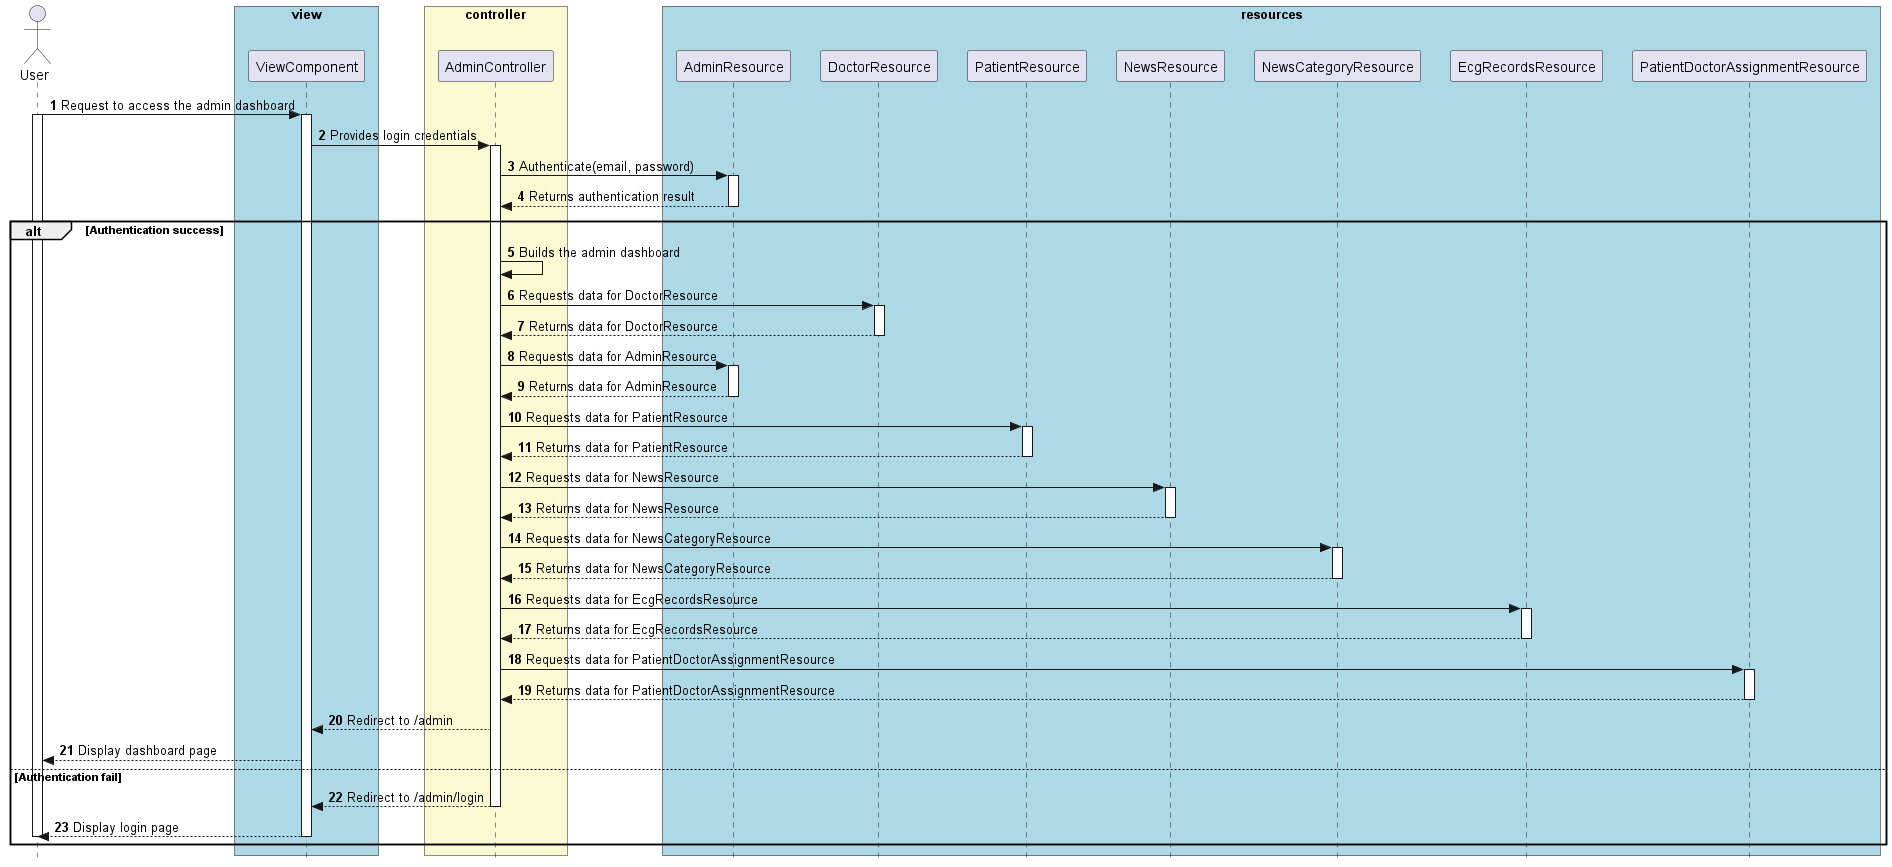
\includegraphics[width=16cm,height=9cm]{Images/server/sequence/web/seq_auth.png}
  \caption[Sơ đồ tuần tự ]{\bfseries \fontsize{12pt}{0pt}
  \selectfont Sơ đồ tuần }
  \label{hinh21} %đặt tên cho ảnh
\end{figure}

\begin{figure}[H]
  \centering
  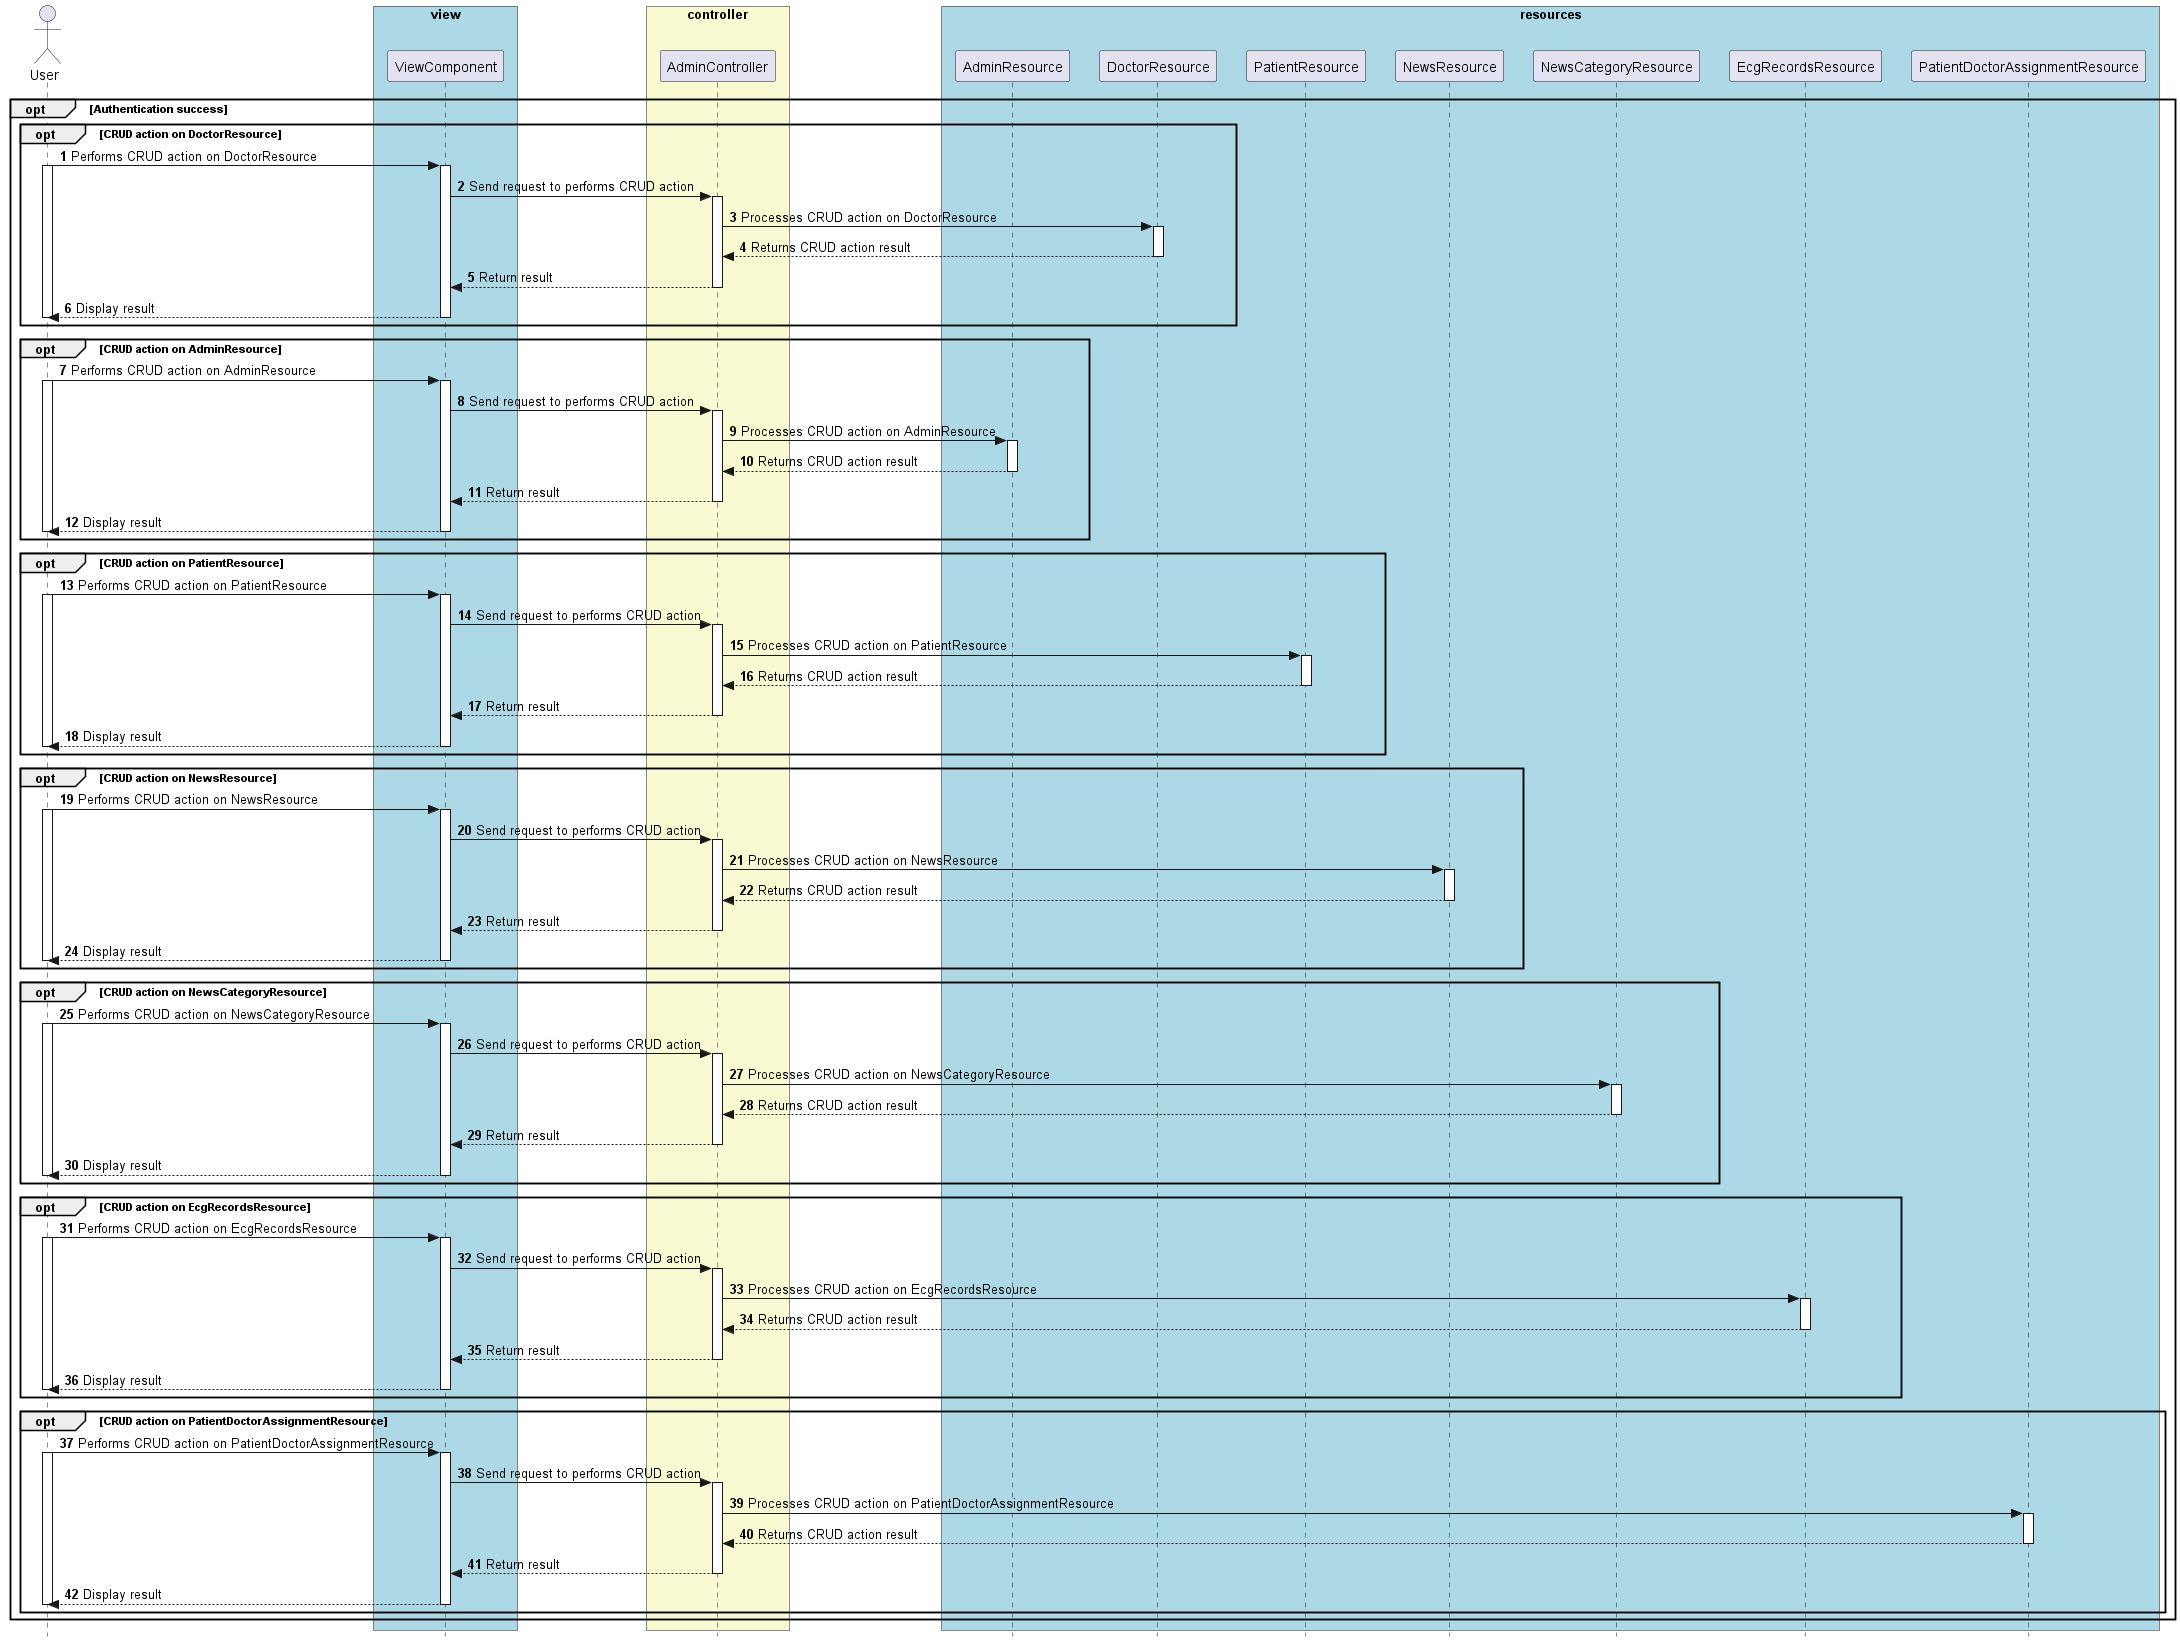
\includegraphics[width=16cm,height=9cm]{Images/server/sequence/web/seq_crud.png}
  \caption[Sơ đồ tuần tự ]{\bfseries \fontsize{12pt}{0pt}
  \selectfont Sơ đồ tuần }
  \label{hinh21} %đặt tên cho ảnh
\end{figure}


\newpage